\documentclass[aspectratio=169]{beamer}

\usepackage{amsmath, amssymb, amsxtra, amsthm, amsfonts}
\usetheme{moloch}
\usecolortheme{beaver}
\setbeamertemplate{footline}
{
  \leavevmode%
  \hbox{%
    \begin{beamercolorbox}[wd=.5\paperwidth,ht=2.25ex,dp=1ex,center]{author in head/foot}%
      \usebeamerfont{author in head/foot}\insertsection
    \end{beamercolorbox}%
    \begin{beamercolorbox}[wd=.5\paperwidth,ht=2.25ex,dp=1ex,right]{date in head/foot}%
      \usebeamerfont{date in head/foot}\inserttitle\hspace*{2em}
      \insertframenumber{} / \inserttotalframenumber\hspace*{2ex}
    \end{beamercolorbox}}%
  \vskip0pt%
}
\makeatother

\usepackage[english]{babel}
\usefonttheme{serif}

\usepackage{mathtools}
\usepackage{graphicx}
\usepackage{bm}
\usepackage{color}
\usepackage[dvipsnames,table]{xcolor}
\usepackage{tikz}
\usepackage{stanli}
\usepackage{verbatim}
\usepackage{tikz}
\usetikzlibrary{shapes,calc,through,3d,patterns}
\usetikzlibrary{decorations.pathreplacing}
\usetikzlibrary{arrows.meta,calc,positioning}

\usepackage{pgfplots}
\usepackage{siunitx} % For formatting numbers
\usepackage{hyperref}
\hypersetup{colorlinks=true,linkcolor=darkred}
\usepackage{multicol}
\usepackage[absolute,overlay,]{textpos}
\usepackage{pgfplots}
\pgfplotsset{width=10cm,compat=1.9}
\usepackage{subcaption}
\usepackage{multirow}
\usepackage{bbding}
\usepackage{arydshln}
\usepackage{mathtools}
\usepackage{tcolorbox}
\usepackage{animate}

\textblockorigin{80mm}{45mm}


\newtheorem{thm}{Theorem}
\newtheorem{cor}[thm]{Corollary}
\newtheorem{prop}[thm]{Proposition}
\newtheorem{lem}[thm]{Lemma}
\theoremstyle{remark}
\newtheorem*{rem}{Remark}

%Block def
\definecolor{darkred}{rgb}{0.6,0,0}
\setbeamertemplate{blocks}[rounded][shadow=false]
\setbeamercolor{block title}{bg=darkred!15,fg=black}
\setbeamercolor{block body}{bg=darkred!5,fg=black}

\setbeamercolor{itemize item}{fg=darkred}
\setbeamercolor{itemize subitem}{fg=darkred}
\setbeamercolor{itemize subsubitem}{fg=darkred}
\setbeamercolor{enumerate item}{fg=darkred}
\setbeamercolor{button}{bg=gray!30,fg=darkred}

\setbeamertemplate{itemize item}[square]
\setbeamertemplate{itemize subitem}[circle]
\setbeamertemplate{itemize subsubitem}[triangle]
\setbeamertemplate{enumerate items}[circle]
\setbeamercolor{item projected}{bg=darkred}

\newcommand{\bolddelta}{\boldsymbol\delta}
\newcommand{\boldxi}{\boldsymbol\xi}
\DeclareMathOperator*{\A}{\text{\raisebox{-0.2cm}{\Huge A}}}




\title{Dynamic analysis of planar beams}
\subtitle{Special structural elements}
\author{ME473 Dynamic finite element analysis of structures}
\institute{Stefano Burzio}
\date{2025}

\begin{document}
\usenavigationsymbolstemplate{}
{\setbeamertemplate{footline}{}

  \frame{\titlepage
    \begin{tikzpicture}[overlay, remember picture]
      \node[anchor=north east, xshift=-.9cm] at (current page.north east) {
\includegraphics[width=2cm]{../images/epfl_logo.png}};
      \node[anchor=south east, xshift=-.87cm, yshift=.05cm] at (current page.south east)  {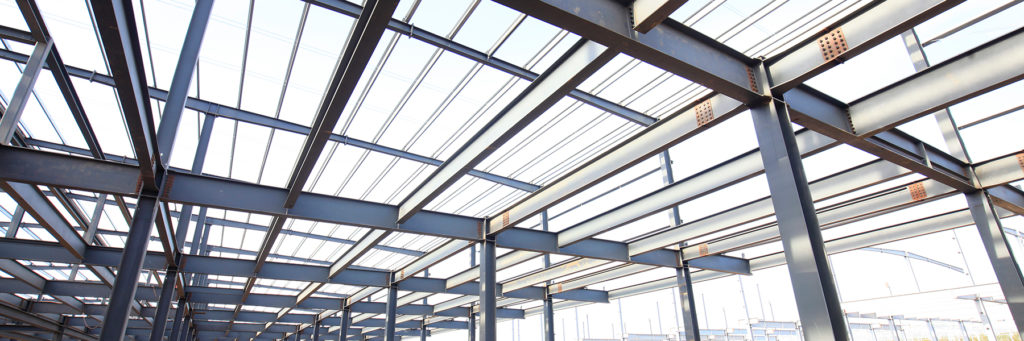
\includegraphics[width=8cm]{../images/frame.png}};
    \end{tikzpicture}
  }

  \begin{frame}{Where do we stand?}
    \begin{center}
      \begin{tabular}{|c|l|l|l|}
        \hline
        \rowcolor{darkred!20}\textbf{Week} & \textbf{Module}                          & \textbf{Lecture topic}             & \textbf{Mini-projects} \\
        \hline

        1                                  & \multirow{5}{7em}{Linear elastodynamics} & Strong and weak forms              &                        \\ \cline{1-1} \cline{3-4}
        2                                  &                                          & Galerkin method                    &                        \\ \cline{1-1} \cline{3-4}
        3                                  &                                          & Finite element method              & Groups formation       \\ \cline{1-1} \cline{3-4}
        4                                  &                                          & Systematization of the procedure   & Project 1 statement    \\
        \cline{1-1} \cline{3-4}
        5                                  &                                          & 3d elements, numerical integration &                        \\
        \hline
        6                                  & \multirow{2}{7em}{Special structural}    & Bars and trusses                   &                        \\
        \cline{1-1} \cline{3-4} 7          &                                          & Planar beams                       & Project 1 submission   \\
                                           & elements                                 &                                    &                        \\

        \hline
      \end{tabular}
    \end{center}
    \vspace{1cm}
  \end{frame}

  \begin{frame}
    \textbf{\large Summary}
    \begin{itemize}
      \item Recap week 6
      \item Euler-Bernoulli beams
      \item Geometric stiffness and buckling
      \item Timoshenko beams
    \end{itemize}
    \vspace{.5cm}

    \textbf{\large Recommended readings}
    \begin{enumerate}
      \item Logan, A first course in the finite element method, 6th ed.
            (chap. 4)
      \item Paz and Leigh, Structural dynamics, 6th ed. (chap. 10)
      \item Ferreira and Fantuzzi, MATLAB Codes for Finite Element Analysis, 2nd ed. (chap. 6 and 10)
    \end{enumerate}
  \end{frame}
}

\section{Recap week 6 \\  Vibrations of bars and trusses}
 {\setbeamercolor{background canvas}{bg=darkred!5}
  \setbeamercolor{block body}{bg=darkred!5,fg=black}

  \begin{frame}{Non-oriented bar element}
    \begin{columns}
      \column{0.5\textwidth}
      \begin{center}
        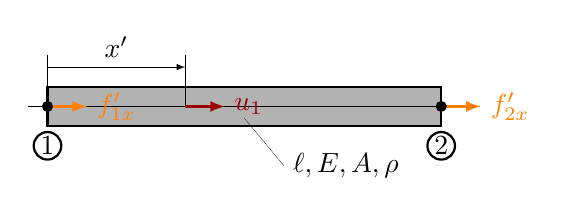
\begin{tikzpicture}[scale=0.5]
          % Draw the rectangle
          \filldraw[fill=gray!60, draw=black,thick] (0,-0.5) rectangle (10,0.5);
          %axis
          \draw[ultra thin] (-0.5,0) -- (10,0);
          %forces
          \draw[thick,-latex,orange] (0,0) -- (1,0) node[right]{$f_{1x}^\prime$};
          \draw[thick,-latex,orange] (10,0) -- (11,0) node[right]{$f_{2x}^\prime$};
          % Mark points
          \fill (0,0) circle (4pt);
          \fill (10,0) circle (4pt);
          \draw[thick] (0,0) ++ (0,-1) circle(0.35cm) node {1};
          \draw[thick] (10,0) ++ (0,-1)  circle(0.35cm) node {2};
          % displacement
          \draw[thick,-latex,darkred] (3.5,0) -- (4.5,0);
          \node[darkred,right] at (4.5,0) {$u_1$};
          % length
          \draw[ultra thin] (3.5,0) -- (3.5, 1.3) ;
          \draw[ultra thin] (0,0) -- (0, 1.3) ;
          \draw[-latex, ultra thin]  (0,1)  to node[sloped,midway,above] {$x^\prime$}(3.5,1) ;
          \draw[ultra thin]  (5,-0.3) -- (6,-1.5) node[right]{$\ell,E,A,\rho$};
        \end{tikzpicture}
      \end{center}

      \column{0.55\textwidth}
      \begin{block}{}
        Differential equation governing the dynamics:
        $$ EA \partial^{2}_{x^\prime x^\prime}u_1(x^\prime, t) = \rho A \ddot{u}_1(x^\prime, t) $$
      \end{block}
    \end{columns}
    \vspace{0.3cm}

    \begin{itemize}
      \item Displacements approximation:
            \[u^h_1(x^\prime,t)=  \mathbf H(x^\prime)\mathbf q_{loc} (t)=\begin{bmatrix}  h_1(x^\prime) & h_2(x^\prime)\end{bmatrix} \begin{bmatrix}  q_{1x}^\prime(t) \\ q_{2x}^\prime(t)\end{bmatrix}\]
      \item Linear local shape functions:
            $$h_1(x^\prime)  =1-\frac{x^\prime}{\ell} \qquad\text{and}\qquad h_2(x^\prime)  =\frac{x^\prime}{\ell}$$
      \item Semi-discrete weak form:
            \[\bolddelta\mathbf{q}_{loc}^T\big(\mathbf{M}_{loc} \ddot{\mathbf{q}}_{loc}(t) + \mathbf{K}_{loc} \mathbf{q}_{loc}(t) - \mathbf{f}_{loc}(t)\big)=0 \]
    \end{itemize}
  \end{frame}

  \begin{frame}{Non-oriented bar element discretization}
    \begin{itemize}
      \item Element stiffness matrix in local coordinates:
            \[ \mathbf{K}_{loc} =\int_0^{\ell}  EA\ \frac{d\mathbf{H}}{dx^\prime}^T\frac{d\mathbf{H}}{dx^\prime}\ dx^\prime =\int_0^{\ell}  EA \begin{bmatrix} (h_1^\prime)^2 & h_1^\prime h_2^\prime \\  h_2^\prime h_1^\prime &  (h_2^\prime)^2 \end{bmatrix} dx^\prime =\frac{EA}{\ell} \begin{bmatrix} 1 & -1 \\ -1 & 1 \end{bmatrix} \]
      \item Element consistent mass matrix in local coordinates:
            \[ \mathbf{M}_{loc} =\int_0^{\ell}  \rho A\ \mathbf{H}^T\mathbf{H}\ dx^\prime =\int_0^{\ell}\rho A \begin{bmatrix} (h_1)^2 &h_1 h_2 \\  h_2 h_1 &  (h_2)^2 \end{bmatrix} dx^\prime =\frac{\rho A\ell }{6} \begin{bmatrix} 2 & 1 \\ 1 & 2 \end{bmatrix} \]
      \item Element applied loads vector in local coordinates:
            \[ \mathbf{f}_{loc}(t) =\begin{bmatrix} h_1(0) \\ h_2(0)\end{bmatrix}f_{1x}^\prime(t) + \begin{bmatrix} h_1(\ell) \\ h_2(\ell)\end{bmatrix}f_{2x}^\prime(t) = \begin{bmatrix} f_{1x}^\prime(t) \\ f_{2x}^\prime(t) \end{bmatrix} \]
    \end{itemize}
  \end{frame}

  \begin{frame}{Arbitrarly oriented bar element}
    \begin{columns}
      \column{0.5\textwidth}
      \begin{itemize}
        \item Displacements in local coordinates:\vspace{-0.3cm}  $$\mathbf{q}_{loc} = [q_{1x}^\prime, q_{2x}^\prime]^T$$
        \item Displacements in global coordinates:\vspace{-0.3cm} $$\mathbf q = [q_{1x},q_{1y},q_{2x},q_{2y}]^T$$
        \item   \textbf{Relation between local and global displacements:}
      \end{itemize}
      \column{0.5\textwidth}
      \begin{center}
        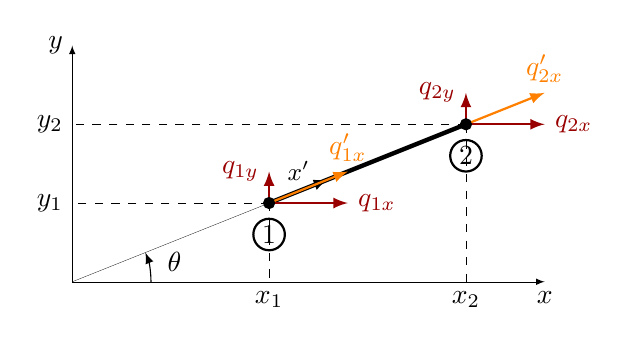
\begin{tikzpicture}[scale=1]
          % Draw background grid
          %\draw[step=1cm,gray,very thin] (0,0) grid (12,6);
          % Define coordinates
          \coordinate (A) at (0,0);
          \coordinate (B) at (2.5,1);
          \coordinate (C) at (5,2);
          % Draw the truss members
          \draw[ultra thin] (A) -- (B);
          \draw[ultra thick] (B) -- (C);
          % Global coordinate system
          \draw[-latex, ultra thin] (0,0) -- (0,3) node[left] {$y$};
          \draw[-latex, ultra thin] (0,0) -- (6,0) node[below] {$x$};
          % Local coordinate systems
          \draw[-latex, darkred,thick] (B) -- ++(0,0.4) node[left] {$q_{1y}$};
          \draw[-latex, darkred,thick] (B) -- ++(1,0) node[right] {$q_{1x}$};
          \draw[-latex, darkred,thick] (C) -- ++(0,0.4) node[left] {$q_{2y}$};
          \draw[-latex, darkred,thick] (C) -- ++(1,0) node[right] {$q_{2x}$};
          % Local primed coordinate system
          \draw[-latex,thick] (B) -- (21.8:3.5) node[midway, above] {\small $x^\prime$};
          % Angles and labels
          \draw[-latex] (1,0) arc (0:21.8:1);
          \node at (1.3,0.25) {$\theta$};
          % Local x' axis
          \draw[-latex, orange, thick] (B) -- ++(1,0.4) node[above] {$q_{1x}^\prime$};
          \draw[-latex, orange, thick] (C) -- ++(1,0.4) node[above] {$q_{2x}^\prime$};
          % Draw supports (circles at joints)
          \filldraw (B) circle (2pt);
          \filldraw (C) circle (2pt);
          % Nodes coord
          \draw[dashed,ultra thin] (B) -- (2.5,0) node[below] {$x_1$};
          \draw[dashed,ultra thin] (B) -- (0,1) node[left] {$y_1$};
          \draw[dashed,ultra thin] (C) -- (5,0) node[below] {$x_2$};
          \draw[dashed,ultra thin] (C) -- (0,2) node[left] {$y_2$};
          % Nodes labels
          \draw[thick] (B) ++ (0,-0.4) circle(0.2cm) node {1};
          \draw[thick] (C) ++ (0,-0.4)  circle(0.2cm) node {2};
        \end{tikzpicture}
      \end{center}
    \end{columns}
    \vspace{0.3cm}
    $$\underbrace{\begin{bmatrix}
          q_{1x}^\prime \\ q_{2x}^\prime
        \end{bmatrix}}_\text{$\mathbf q_{loc}$}=\underbrace{\begin{bmatrix}
          \cos(\theta) & \sin(\theta) & 0            & 0            \\
          0            & 0            & \cos(\theta) & \sin(\theta)
        \end{bmatrix}}_\text{$\mathbf T$}\underbrace{\begin{bmatrix}
          q_{1x} \\ q_{1y} \\ q_{2x} \\ q_{2y}
        \end{bmatrix}}_\text{$\mathbf q$}
    $$
  \end{frame}

  \begin{frame}{Discretization of arbitrarly oriented bar}
    \begin{itemize}
      \item Element stiffness matrix in global coordinates:
            $$\mathbf{K} = \mathbf T^T \mathbf{K}_{loc} \mathbf T   =\frac{EA}{\ell}\begin{bmatrix}
                \cos^2(\theta) & \sin(\theta)\cos(\theta) & -\cos^2(\theta)           & -\sin(\theta)\cos(\theta) \\
                               & \sin^2(\theta)           & -\sin(\theta)\cos(\theta) & -\sin^2(\theta)           \\
                               &                          & \cos^2(\theta)            & \sin(\theta)\cos(\theta)  \\
                \text{Symm.}   &                          &                           & \sin^2(\theta)            \\
              \end{bmatrix}$$
      \item Element consistent mass matrix in global coordinates:
            $$\mathbf{M} = \mathbf T^T \mathbf{M}_{loc} \mathbf T =\frac{\rho A\ell}{6}\begin{bmatrix}
                2\cos^2(\theta) & 2\sin(\theta)\cos(\theta) & \cos^2(\theta)           & \sin(\theta)\cos(\theta)  \\
                                & 2\sin^2(\theta)           & \sin(\theta)\cos(\theta) & \sin^2(\theta)            \\
                                &                           & 2\cos^2(\theta)          & 2\sin(\theta)\cos(\theta) \\
                \text{Symm.}    &                           &                          & 2\sin^2(\theta)           \\
              \end{bmatrix}
            $$
    \end{itemize}
  \end{frame}

  \begin{frame}{Illustrative example}
    \begin{block}{}
      \textbf{Plane truss:} structure composed of oriented bar elements that all lies in a common plane and are connected by frictionless pins.
    \end{block}
    \vspace{0.3cm}
    \begin{columns}
      \begin{column}{.45\textwidth}
        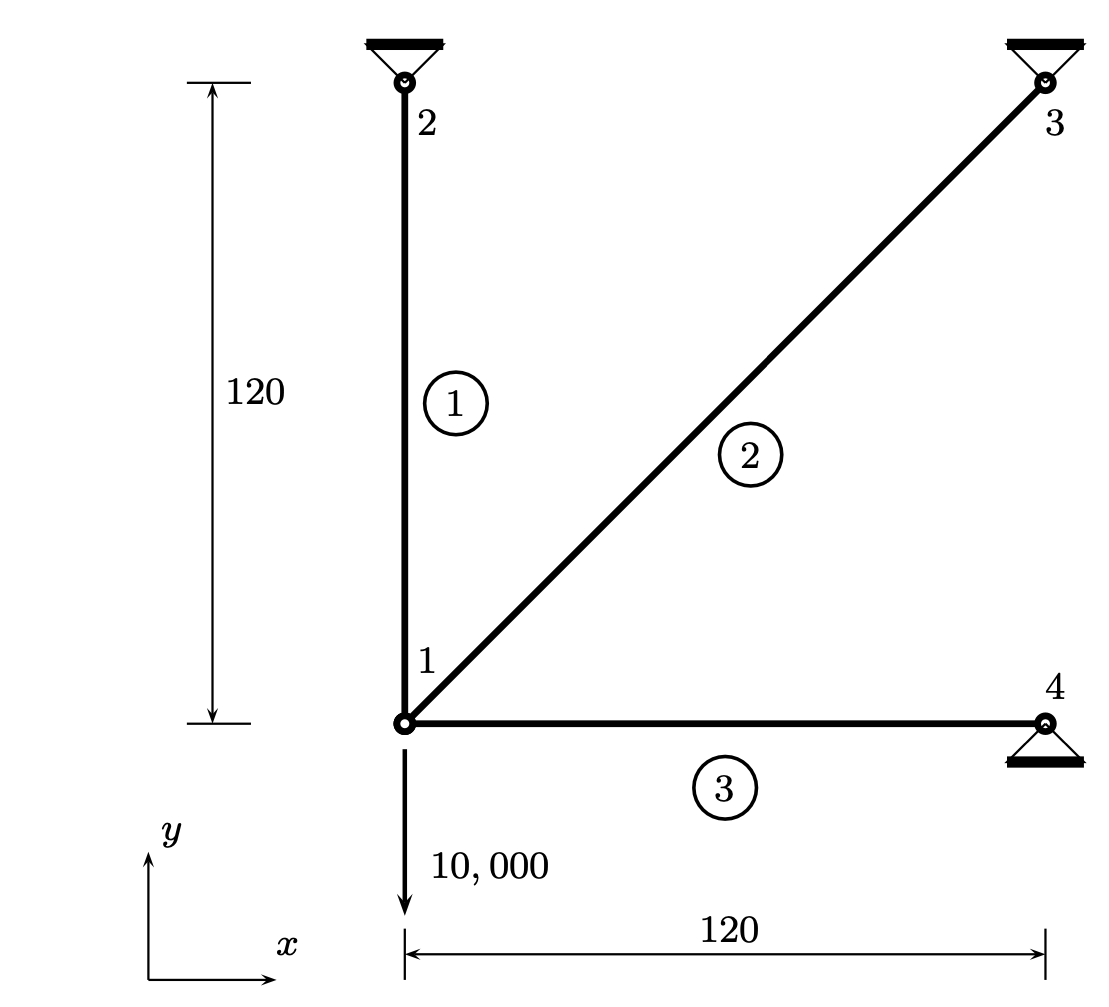
\includegraphics[width=4.5cm]{../images/trussExample.png}
      \end{column}

      \begin{column}{.6\textwidth}
        \small \begin{tabular}{c|c|c|c}
          Elements & Nodes & ${}^e\theta$  & ${}^e\ell$       \\
          \hline
          1        & 1,\ 2 & $90^{\circ}$  & $120$ mm         \\
          2        & 1,\ 3 & $45^{\circ} $ & $120\sqrt{2}$ mm \\
          3        & 1,\ 4 & $0^{\circ} $  & $120$ mm         \\
        \end{tabular}

        \vspace{0.2cm}
        Elementary stiffness and mass matrices:
        $$\begin{aligned}
            {}^e\mathbf K & = {}^e\mathbf T\mathbf K_{loc}{}^e\mathbf T \\
            {}^e\mathbf M & = {}^e\mathbf T\mathbf M_{loc}{}^e\mathbf T
          \end{aligned}\hspace{1.5cm} e=1,2,3$$
      \end{column}
    \end{columns}
    \begin{block}{}
      Global stiffness and mass matrices: $\mathbf K = \A_{e=1}^3 {}^e\mathbf K$ and $\mathbf M = \A_{e=1}^3 {}^e\mathbf M$.
    \end{block}
  \end{frame}
 }

\section{Euler-Bernoulli planar beams}

\begin{frame}{What is a beam?}
  \begin{itemize}
    \item Considered to be a uniaxial (slender) element: the longitudinal direction is sufficiently larger than the other two.
    \item Cross-section does not change along the element's length.
    \item Subjected to \textbf{transversal loading} that produced significant bending effects.
    \item Very common type of structures used in steel buildings, bridges, towers, etc...
  \end{itemize}
  \begin{center}
    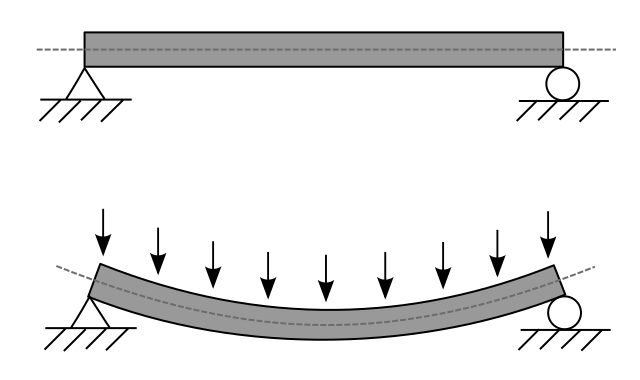
\includegraphics[height=3cm]{../images/beam.png}
  \end{center}
\end{frame}

\begin{frame}{Euler-Bernoulli beam assumptions}
  \begin{columns}
    \column{0.4\textwidth}
    \begin{center}
      \vspace{-1cm}
      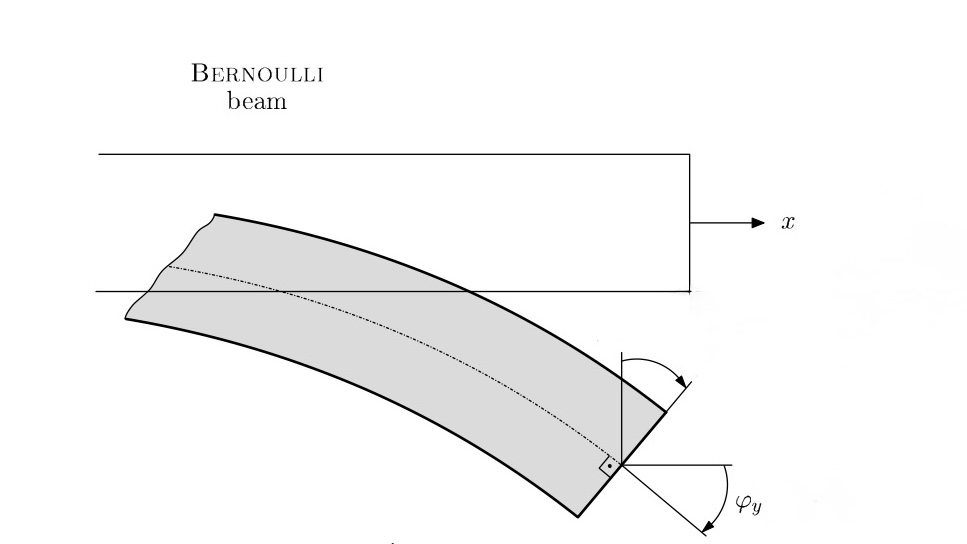
\includegraphics[height=3.5cm]{../images/beamBern.jpeg}
    \end{center}
    \column{0.6\textwidth}
    \textbf{Thin beam theory}
    \begin{itemize}
      \item Planar cross section perpendicular to the longitudinal centroidal axis of the beam remains \textbf{planar} and \textbf{perpendicular} to the longitudinal axis after bending occurs.
      \item Shear deformations $\varepsilon_{12}$ of the planar cross section  are neglected.
      \item The beam cross-section is infinitely rigid in its own plane.
      \item Reasonable model for slender structures made of isotropic materials.
    \end{itemize}
  \end{columns}
\end{frame}

\begin{frame}{Euler-Bernoulli beam assumptions}
  \textbf{Valid for:} slender beams ($h/\ell<1/100$).
  \begin{center}
    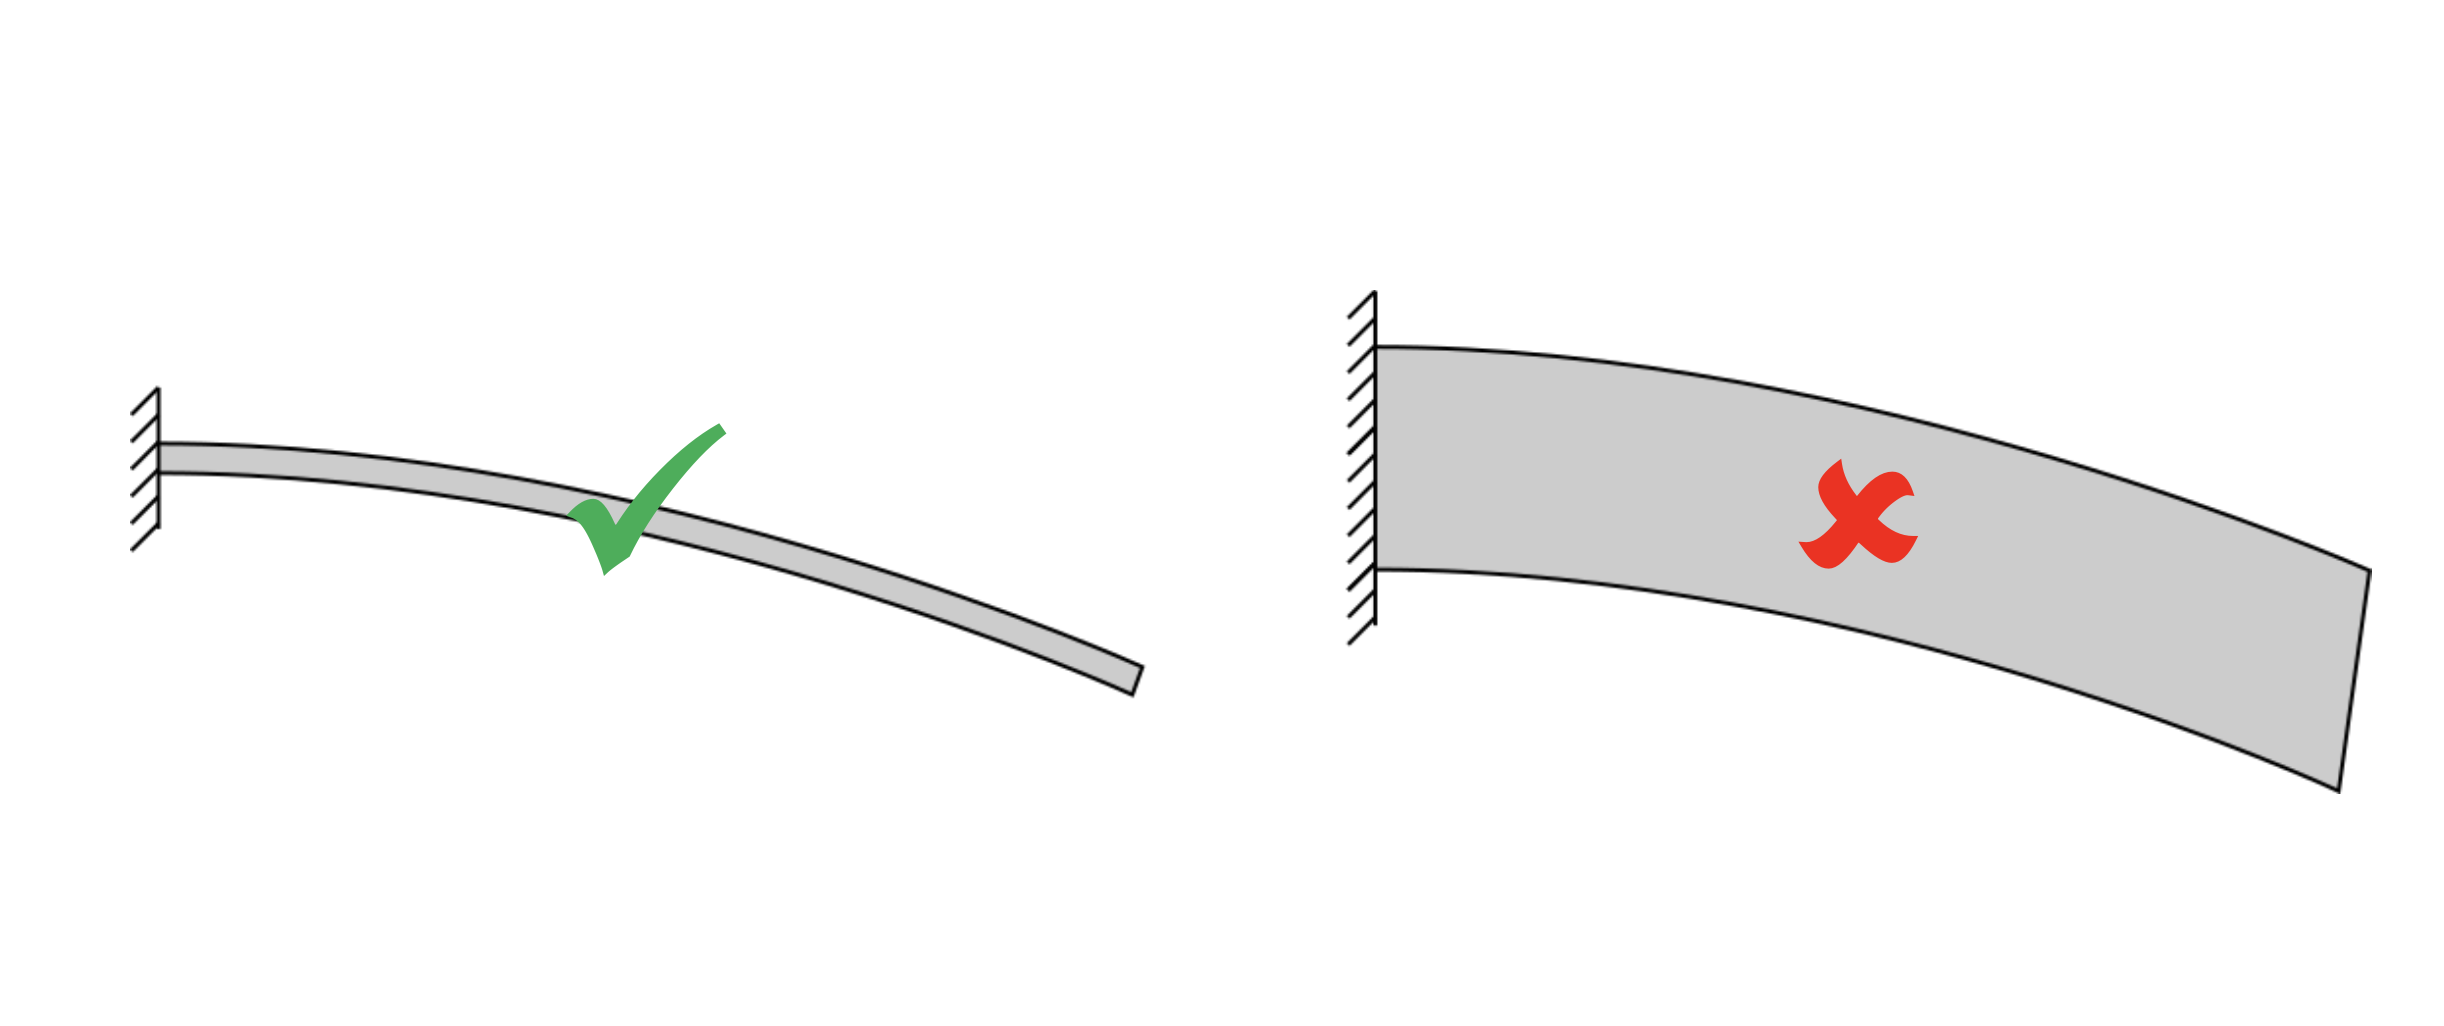
\includegraphics[height=5cm]{../images/eulerBeam.png}
  \end{center}
  {\footnotesize (Credit:
  \hyperlink{https://ethz.ch/content/dam/ethz/special-interest/baug/ibk/structural-mechanics-dam/education/femI/2024/Lecture_1_EC_2024.pdf}{Chatzi and Egger})}
\end{frame}

\begin{frame}{Timoshenko beam assumptions}
  \begin{columns}
    \column{0.4\textwidth}
    \begin{center}
      \vspace{-0.5cm}
      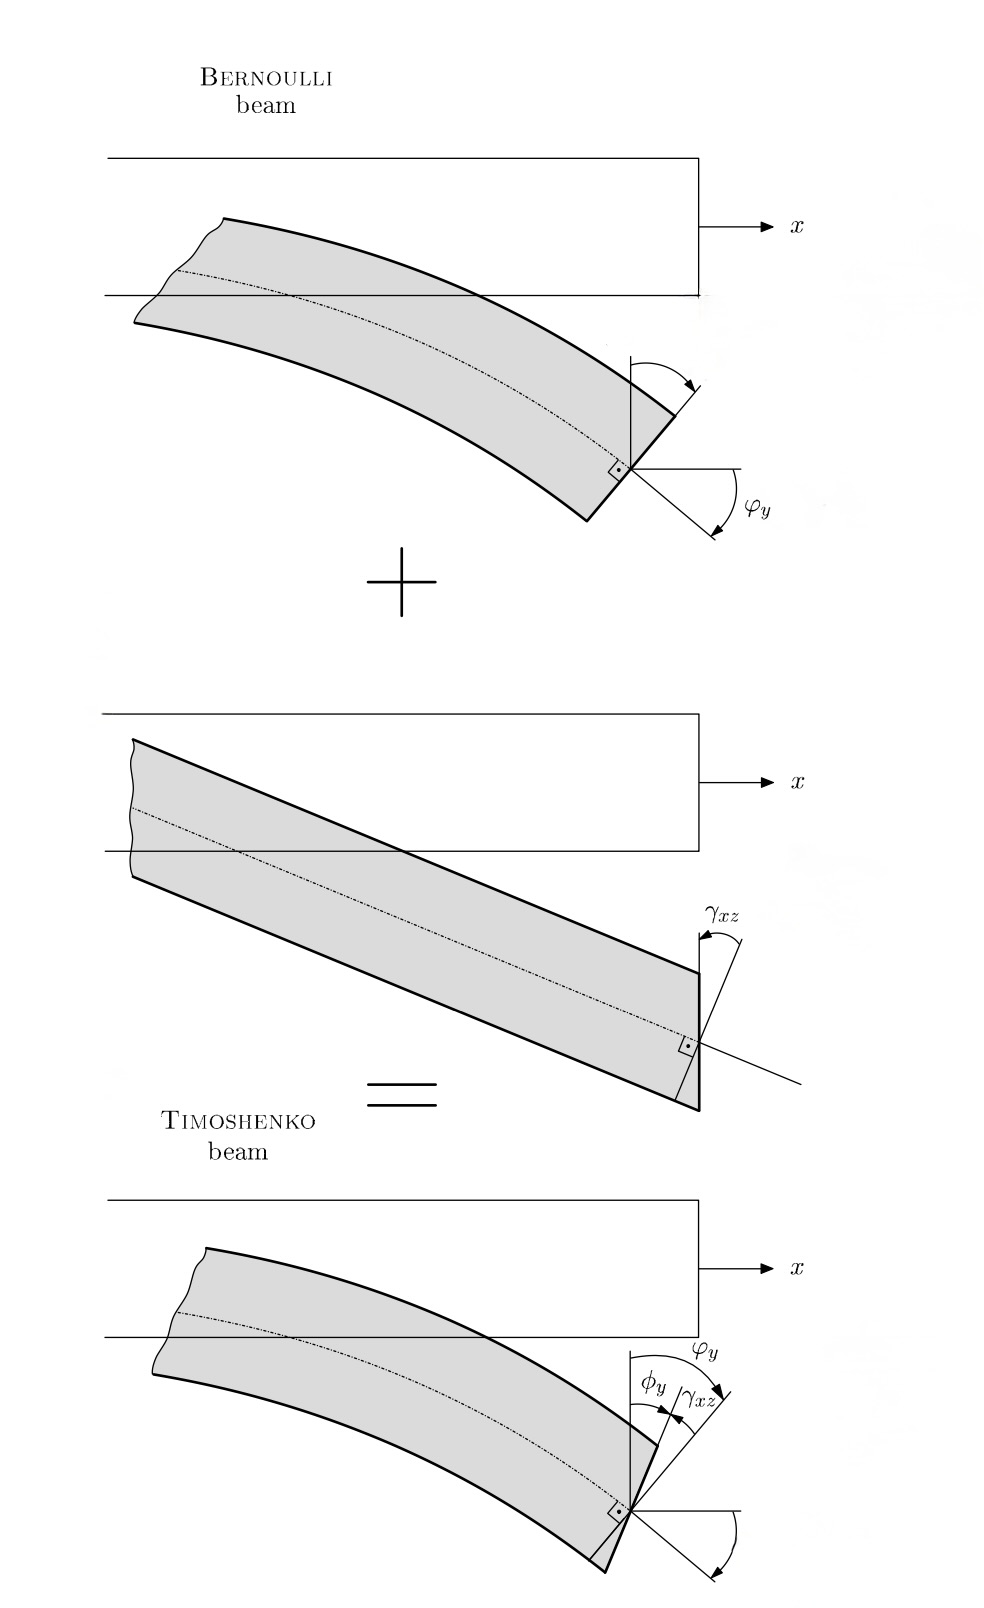
\includegraphics[height=7cm]{../images/beamTimoBern.jpeg}
    \end{center}
    \column{0.6\textwidth}
    \textbf{Thick beam theory}
    \begin{itemize}
      \item Planar cross section perpendicular to the longitudinal centroidal axis of the beam remains \textbf{planar} but \textbf{not necessarily perpendicular} to the longitudinal beam axis after bending occurs.
      \item Shear deformations $\varepsilon_{12}$ of the planar cross section  are considered.
      \item Reasonable model for beams made of composite material that require the shear effect account.
    \end{itemize}
  \end{columns}
\end{frame}

\begin{frame}{Timoshenko beam assumptions}
  \textbf{Valid for:} slender beams ($h/\ell<1/100$) and thick beams ($h/\ell>1/10$).

  \begin{center}
    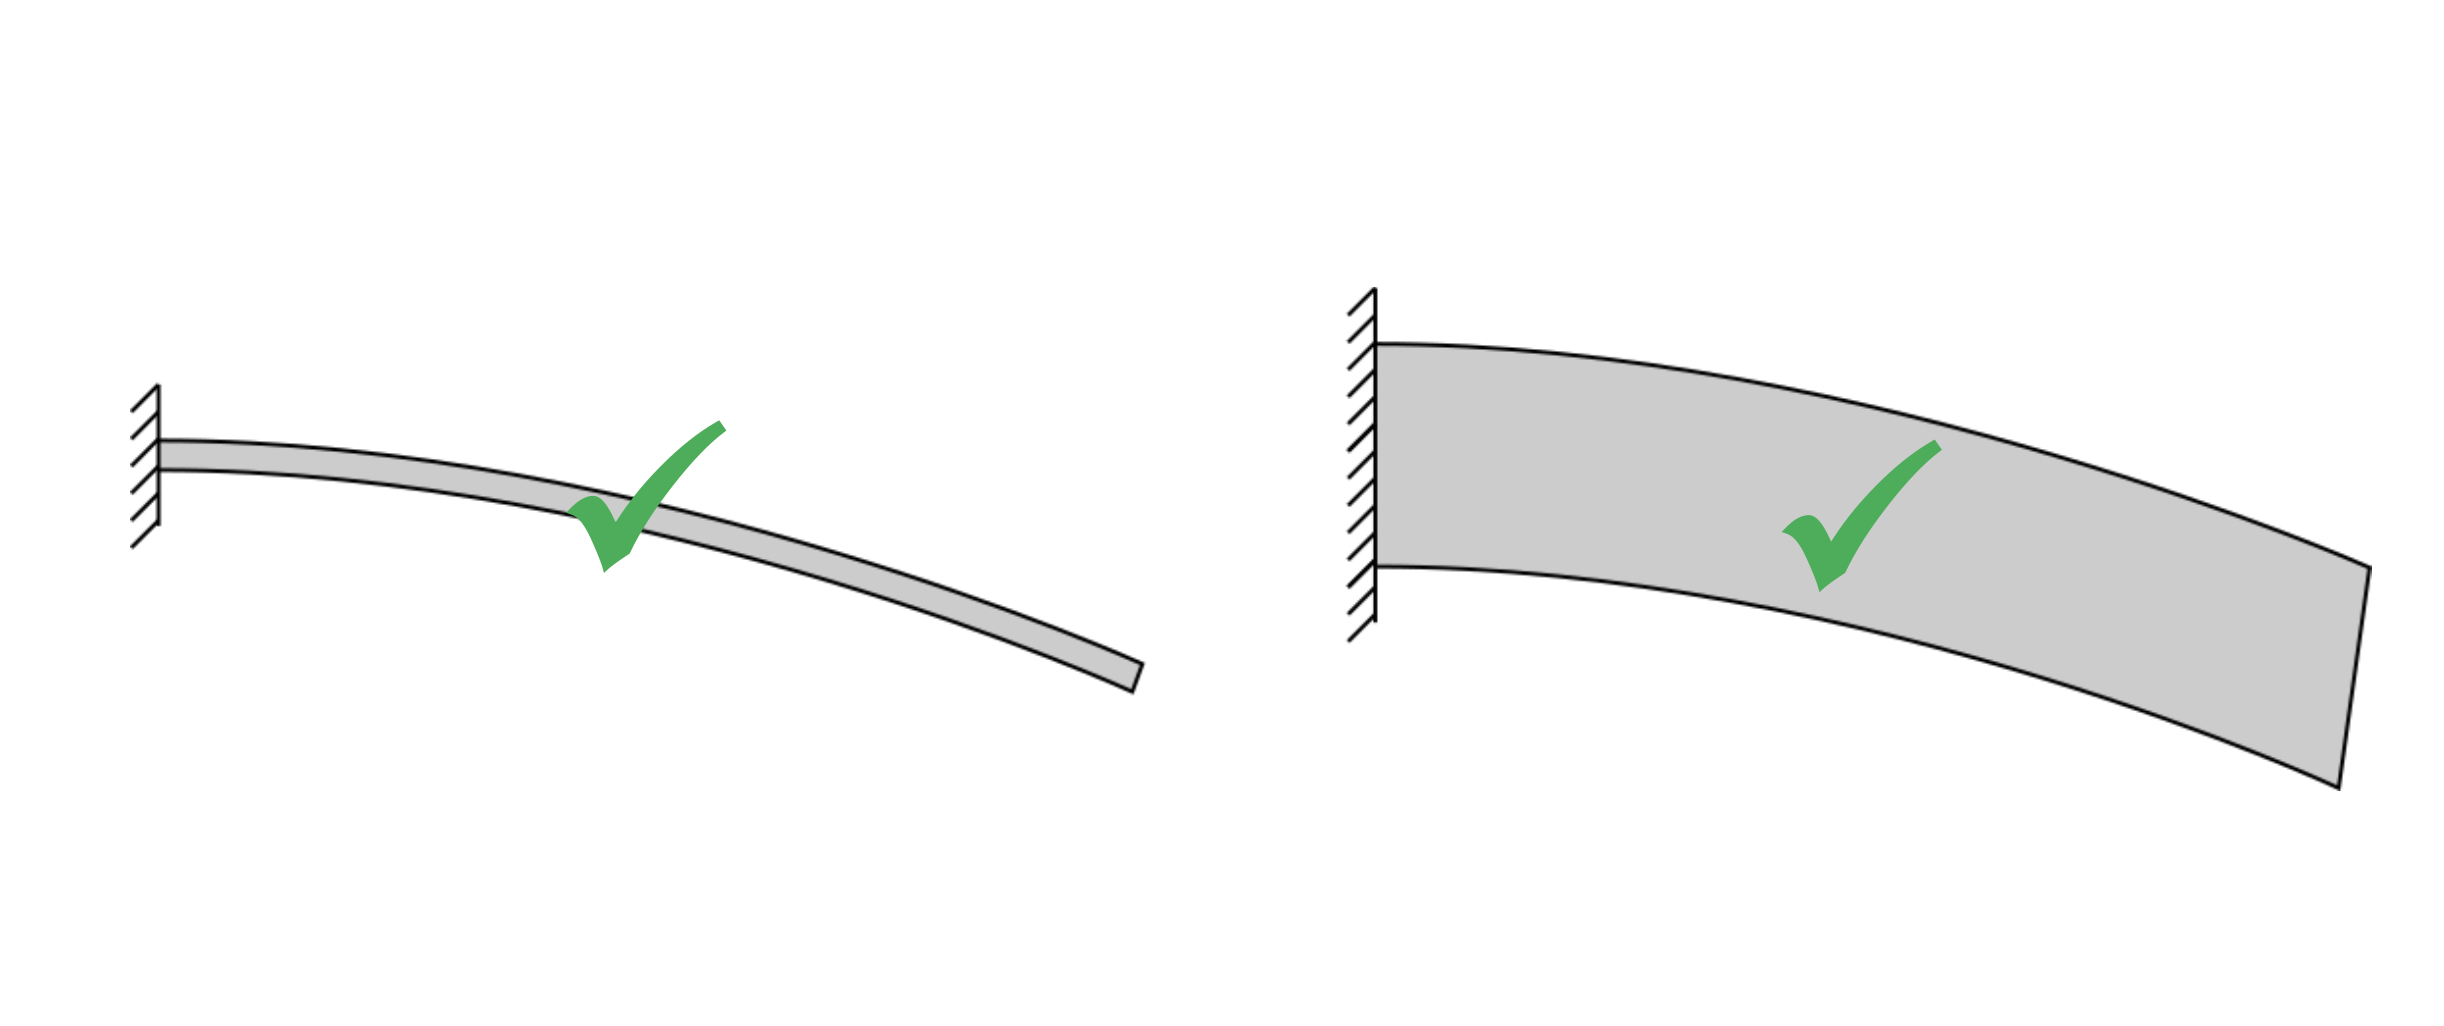
\includegraphics[height=5cm]{../images/timoBeam.png}
  \end{center}
  {\footnotesize (Credit:
  \hyperlink{https://ethz.ch/content/dam/ethz/special-interest/baug/ibk/structural-mechanics-dam/education/femI/2024/Lecture_1_EC_2024.pdf}{Chatzi and Egger})}
\end{frame}

\begin{frame}
  \frametitle{Kinematic assumptions for planar Euler-Bernoulli beam}
  \begin{enumerate}
    \item The beam dynamics will be restricted to the $O(x,y)$ plane.
    \item The beam cross-section remains planar after deformation.
    \item Lines that are straight and perpendicular to the beam axis remain straight and perpendicular during deformation.
  \end{enumerate}

  \begin{columns}
    \column{0.6\textwidth}
    \begin{center}
      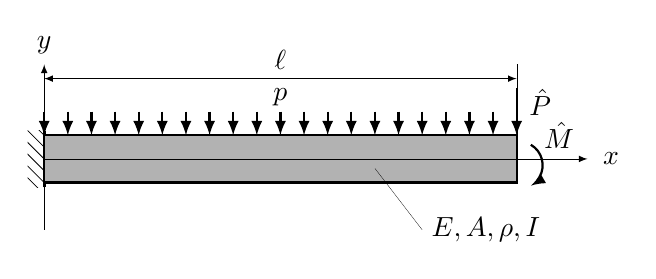
\begin{tikzpicture}[scale=0.6]
        \point{a}{0}{0.3};
        \support {3}{a}[270];
        % Draw the rectangle
        \filldraw[fill=gray!60, draw=black,thick] (0,0) rectangle (10,1);
        % Add the p vector
        \foreach \i in {0,...,19}
          {
            \draw[-latex, thick]  (0.5*\i,1.5)--(0.5*\i,1);
          }
        \node at (5,1.8) {\(p\)};
        %axis
        \draw[-latex, ultra thin] (0,0.5) -- (11.5,0.5);
        \draw[-latex, ultra thin] (0,-1) -- (0,2.5);
        \node at (12,0.5) {\(x\)};
        \node at (0,2.9) {\(y\)};
        % length
        \draw[ultra thin] (10,0) -- (10, 2.5) ;
        \draw[latex-latex, ultra thin]  (0,2.2)  to node[sloped,midway,above] {$\ell$}(10,2.2) ;
        % M and V 
        \draw[-latex, thick] (10.3,0.8) arc (60:-60:0.5);
        \node at (10.5,1.7) {\(\hat P\)};
        \draw[-latex, thick] (10,2) -- (10,1);
        \node at (10.9,1) {\(\hat M\)};
        \draw[ultra thin]  (7,0.3) -- (8,-1) node[right]{$E,A,\rho,I$};
      \end{tikzpicture}
    \end{center}
    \column{.25\textwidth}
    {\tiny Model parameters:
      \begin{itemize}\setlength\itemsep{0.05em}
        \item $A$ cross-sectional area
        \item $E$ Young's modulus
        \item $\rho$ material density
        \item $I$ moment of inertia
        \item $\ell$ length
      \end{itemize}}
    \column{.25\textwidth}
    {\tiny Loads:
      \begin{itemize}\setlength\itemsep{0.05em}
        \item  $\hat M$  bending moment \\ at free end
        \item  $\hat P$ load at \\ free end
        \item $p$ distributed transversal load
      \end{itemize}
    }
  \end{columns}
  \begin{block}{Variables:}
    \begin{multicols}{2}
      \begin{itemize}\setlength\itemsep{0.05em}
        \item $u_{1}(x,t)$ axial displacement
        \item $u_{2}(x,t)$ transversal displacement\vspace{.1cm}
      \end{itemize}
    \end{multicols}
  \end{block}
\end{frame}

\begin{frame}
  \frametitle{Displacements field}
  Introduce an auxiliary variable $\theta_{3}(x,t)$ representing the total rotation of the section around the $Oz$ axis. Rotations are positive in clockwise direction.
  \begin{columns}
    \column{0.35\textwidth}
    \begin{center}
      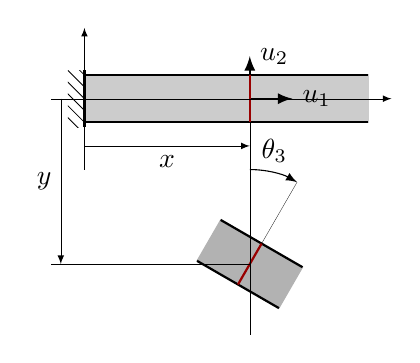
\begin{tikzpicture}[scale=0.6]
        \point{a}{0}{0.3};
        \support {3}{a}[270];
        % Draw the rectangle
        \filldraw[fill=gray!40, draw=gray!40,thick] (0,0) rectangle (6,1);
        \draw[thick](6,1)-- (0,1) -- (0,0)--(6,0);
        \draw[-latex,thick] (3.5,0.5) -- (4.4,.5) node[right]{$u_{1}$};
        \draw[-latex,thick] (3.5,0.5) -- (3.5,1.4) node[right]{$u_{2}$};
        \draw[darkred,thick] (3.5,0) -- (3.5,1);
        %deformed 
        \filldraw[fill=gray!60,draw=gray!60, rotate around={-30:(3.5,-3)}] (2.5,-2.5) rectangle (4.5,-3.5);
        \draw[thick,rotate around={-30:(3.5,-3)},shift={(0,-0.5)}](2.5,-3)-- (4.5,-3);
        \draw[thick,rotate around={-30:(3.5,-3)},shift={(0,0.5)}](2.5,-3)-- (4.5,-3);
        \draw[ultra thin,rotate around={-30:(3.5,-3)}](3.5,-3)-- (3.5,-1);
        \draw[darkred,thick,rotate around={-30:(3.5,-3)}](3.5,-2.5)-- (3.5,-3.5);
        \draw[-latex] (3.5,-1) arc (90:60:2) node[midway,above] {$\theta_{3}$};
        %x1 and x2
        \draw[ultra thin] (3.5,-0.7) -- (3.5,0);
        \draw[-latex,ultra thin] (0,-0.5) to node[midway,below] {$x$} (3.5,-.5);
        \draw[ultra thin]  (-.7,-3)-- (3.5,-3);
        \draw[ultra thin] (3.5,-4.5) -- (3.5,-0.5);
        \draw[ultra thin] (-.7,0.5) -- (0,0.5);
        \draw[-latex,ultra thin] (-.5,.5) to node[midway,left] {$y$} (-.5,-3);
        %axis
        \draw[ultra thin,-latex] (0,0.5) -- (6.5,0.5);
        \draw[ultra thin,-latex] (0,-1) -- (0,2);
      \end{tikzpicture}
    \end{center}
    \column{0.7\textwidth}

    \begin{itemize}
      \item The first Euler-Bernoulli assumption implies
            $$u_3=0.$$
      \item The second Euler-Bernoulli assumption implies
            $$u_{1}=-y\theta_{3}\qquad\qquad\text{\emph{(rotation-axial displ.)}}$$
            %Notice, that because the convention of positive rotations in the counterclockwise directions, the term has a negative sign. In this way, is assured that a positive value of rotation will create a negative axial displacement for a positive $y$.
      \item The third Euler-Bernoulli assumption implies
            $$\theta_{3}=\partial_{x}u_{2}\qquad\text{\emph{(rotation-transversal displ.)}}$$
            %rotation of the cross- section beam must be equal to the slope of the beam axis,
    \end{itemize}
  \end{columns}
  \begin{block}{}
    \textbf{Only one unknown:} transversal displacement $u_{2}(x,t)$.
  \end{block}
\end{frame}

\begin{frame}
  \frametitle{Stress, strain and displacement fields}
  \begin{block}{Strain-displacement relationships}
    Substituting the displacement field $\mathbf u$ into $\boldsymbol{\varepsilon}=\nabla\mathbf u$ yield to :
    \vspace{-0.6cm}

    \begin{align*}
      \varepsilon_{11} & =\partial_{x}u_{1}=-y\partial_{xx}^2u_{2}                           & \varepsilon_{22}       & =\partial_{y}u_{2}=0                      \\
      \varepsilon_{12} & =\partial_{x}u_{2}+\partial_{y}u_{1}=\partial_{x}u_{2}-\theta_{3}=0 & \quad \varepsilon_{33} & = \varepsilon_{23} = \varepsilon_{13} = 0
    \end{align*}
  \end{block}
  \begin{block}{Generalized Hooke's law}
    Using the linear relationship for homogeneous and isotropic material,
    $\boldsymbol\sigma=\mathbf C\boldsymbol\varepsilon$, is possible to write the stress field in term of the strain field as :
    \vspace{-0.6cm}

    \begin{align*}
      \sigma_{11}       & =(\lambda + 2G)\varepsilon_{11} &
      \sigma_{22}       & =\lambda \varepsilon_{11}         \\
      \sigma_{33}       & =\lambda \varepsilon_{11}       &
      \quad \sigma_{12} & = \sigma_{13} = \sigma_{23} = 0
    \end{align*}

    where $\lambda=\frac{E}{(1+\nu)(1-2\nu)}$ and the shear modulus $G=\frac{E}{2(1+\nu)}$ are Lamé constants.
  \end{block}
\end{frame}

\begin{frame}{Dynamic equilibrium equations}
  The theoretical stresses do not agree well with the experimental measurements.

  \begin{block}{Additional assumptions regarding the stress field}
    $$\sigma_{11}  = E\varepsilon_{11}, \qquad\text{and}\qquad
      \sigma_{22}  =  \sigma_{33} =  \sigma_{12} = \sigma_{13} = \sigma_{23} = 0.
    $$
    \small \emph{Justification} : the dimension of the cross-section is much smaller that the beam length.
  \end{block}

  \begin{columns}
    \column{0.5\textwidth}
    \begin{center}
      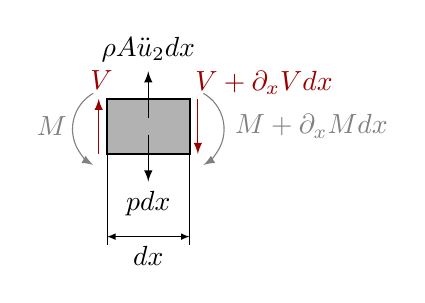
\begin{tikzpicture}[scale=0.35]
        % Draw the rectangle
        \filldraw[fill=gray!60, draw=black,thick] (0,0) rectangle (3,2);
        %axis
        \draw[ultra thin] (0,0) -- (0,-3.3);
        \draw[ultra thin] (3,0) -- (3,-3.3);
        \draw[latex-latex,ultra thin] (0,-3) to node[midway,below] {$dx$} (3,-3);
        \draw[-latex]  (1.5,1.3)  -- (1.5,3) node[above] {$\rho A\ddot u_{2}dx$};
        \draw[-latex]  (1.5,.7)  -- (1.5,-1) node[below] {$pdx$};
        \draw[gray,-latex] (-0.5,2.2) arc (120:240:1.5);
        %M vactors 
        \node[gray] at (-2,1) {\(M\)};
        \draw[gray,-latex] (3.5,2.2) arc (60:-60:1.5);
        \draw (4.3,1) node[gray,right] {$M+\partial_{x}Mdx$};
        % Add the V vectors
        \draw[darkred,-latex] (-0.3,0) -- (-0.3,2);
        \node[darkred,above] at (-0.2,2) {\(V\)};
        \draw[darkred,latex-] (3.3,0) -- (3.3,2);
        \node[darkred,above] at (5.7,1.8) {\(V+\partial_{x}Vdx\)};
      \end{tikzpicture}
    \end{center}
    \column{0.6\textwidth}
    \small
    \vspace{-0.5cm}
    \begin{itemize}
      \setlength\itemsep{-5pt}
      \item Equilibrium of transverse forces:
            $$ \partial_{x}{\color{darkred}V}+p =\rho A\ddot u_{2}$$
      \item Equilibrium of moments:
            $$ \partial_{x}{\color{gray}M}+{\color{darkred}V}=0$$
    \end{itemize}
  \end{columns}
  \vspace{-0.3cm}
  $${\color{gray}M} =-\int_{A} y\sigma_{11}\, dA=-\int_{A}yE\varepsilon_{11}\, dA={\color{gray}EI\partial_{xx}^2u_{2}}$$
\end{frame}

\begin{frame}
  \frametitle{Strong form for transversal vibrations for Euler-Bernoulli beam}
  The strong form consists of finding the transversal displacement $u_{2}\in C^4([0,\ell]\times[0,T])$ such that the following equilibrium equation is satisfied:
  \begin{block}{}
    $$\partial_{xx}^2\big(EI\partial_{xx}^2u_{2}\big)+\rho A\ddot u_{2}=p.$$
  \end{block}
  Coupled with four boundary conditions:
  \begin{block}{}
    \vspace{-0.5cm}
    \begin{align*}
      u_2(0,t)                                             & =0       &
      \partial_x\left(-EI\partial_{xx}^2u_2\right)(\ell,t) & = \hat P   \\
      \partial_{x}u_{2}(0,t)                               & =0       &
      \quad EI\partial_{xx}^2u_{2}(\ell,t)                 & = \hat M
    \end{align*}
  \end{block}
  and two initial conditions:
  \begin{block}{}
    $$u_2(x,0)=u_{0}(x)\qquad \dot u_2(x,0)=v_{0}(x)$$
  \end{block}
\end{frame}


\begin{frame}
  \frametitle{Weak form for transversal vibrations for Euler-Bernoulli beam}
  Find the transversal displacement $u_{2}\in \mathcal U$ such that the following equation is satisfied for every virtual transversal displacement $\delta u_2\in \mathcal V$:
  \begin{block}{}
    \vspace{-0.5cm}\[
      \int_0^\ell EI\, \partial_{xx}^2 u_2 \, \partial_{xx}^2 \delta u_2 \, dx + \int_0^\ell \rho A\, \ddot u_2 \, \delta u_2 \, dx = \int_0^\ell p\, \delta u_2 \, dx + \hat M\, \delta u_2'(\ell) + \hat P\, \delta u_2(\ell)
    \]

    \vspace{-0.5cm}
    \begin{align*}
      \mathcal U & =\big\{u_2(\cdot,t)\in H^2(]0,\ell[)\ |\ u_2(0,t)=\partial_{x}u_{2}(0,t)=0\ \forall t\in]0,T[\big\} \\
      \mathcal V & =\big\{\delta u_2\in H^2(]0,\ell[)\ |\ \delta u_2(0)=\delta u_{2}^\prime(0)=0 \big\}
    \end{align*}
  \end{block}
  \vspace{0.2cm}
  The Sobolev space $H^2(]0,\ell[)$ is the defined as:
    $$H^2(]0,\ell[)=\Big\{f\in L^2(]0,\ell[)\ |\ \int_0^l \big(\partial_{x}f(x)\big)^2 \ dx<\infty, \ \int_0^l \big(\partial_{xx}^2f(x)\big)^2 \ dx<\infty  \Big\}.$$
\end{frame}

\begin{frame}{Approximated transversal displacement}
  \begin{itemize}
    \item Euler-Bernoulli theory states that both transversal displacement $u_2$ and rotation $\theta_{3}=\partial_{x}u_{2}$ must be differentiable within finite elements and continuous between elements.
    \item Shape functions that meet this requirement are said to have $\mathbf{C^1}$ \textbf{continuity}.
  \end{itemize}
  \begin{center}
    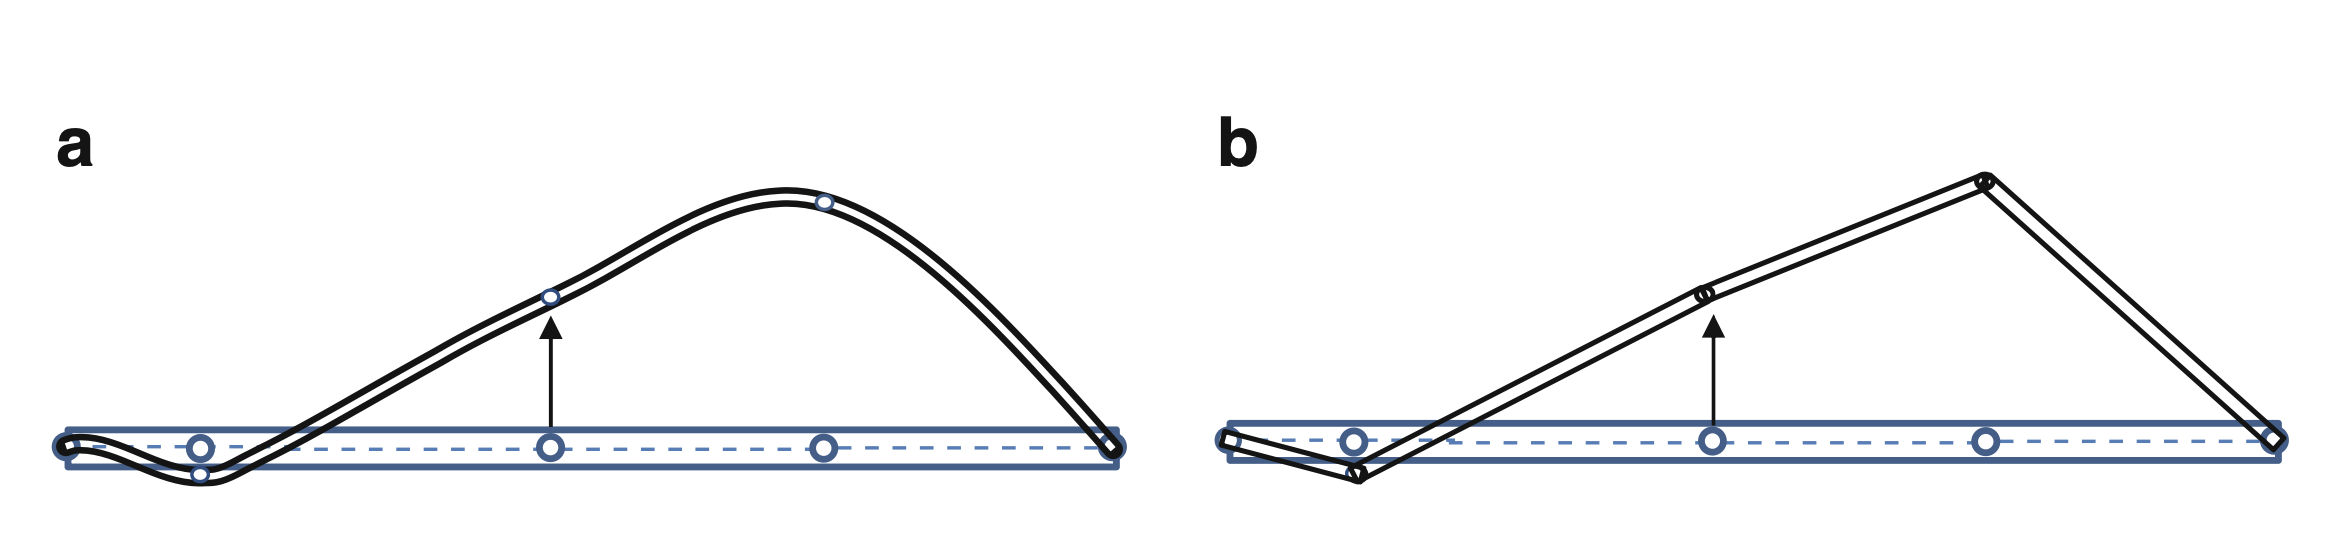
\includegraphics[height=2cm]{../images/c1cont.png}
    \\
    Cubic vs. linear elements.   \noindent{\tiny\emph{Credit: [N]}}
  \end{center}
  \begin{tcolorbox}[colback=darkred!10,colframe=darkred!40!black]
    \textbf{Assume the approximated transversal displacement to be}
    {\color{darkred}$$u_2^h(x,t)=a_3(t)x^3 +a_2(t)x^2 + a_1(t)x  + a_0(t)$$}
    \vspace{-0.7cm}
  \end{tcolorbox}
\end{frame}

\begin{frame}{Nodal degrees of freedom within a beam element}
  \vspace{-0.5cm}
  \begin{columns}
    \column{0.35\textwidth}
    \begin{center}
      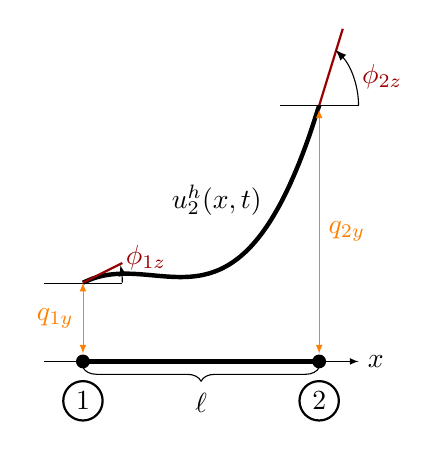
\begin{tikzpicture}[scale=1]
        % Define points
        \coordinate (A) at (0, 0);
        \coordinate (B) at (3, 0);
        % Mark points
        \fill (A) circle (2.5pt);
        \fill (B) circle (2.5pt);
        % Label the element
        \draw[ultra thick] (A) --(B);
        \draw[thick] (A) ++ (0,-0.5) circle(0.25cm) node {1};
        \draw[thick] (B) ++ (0,-0.5)  circle(0.25cm) node {2};
        %Axis 
        \draw[-latex,ultra thin] (-0.5,0) --(3.5,0) node[right]{$x$};
        %Draw function
        \draw[ultra thick,domain=0:3, smooth, variable=\x]
        plot ({\x}, {(1+0.5*\x-2*\x*\x/3+1*\x*\x*\x/4)});
        \draw[thick,darkred,domain=0:0.5, smooth, variable=\x]
        plot ({\x}, {(1+0.5*\x)});
        \draw[thick,darkred,domain=3:3.3, smooth, variable=\x]
        plot ({\x}, {(3.25*\x-6.5)});
        \node[above=1pt] at (1.7, 1.7) {$u_2^h(x,t)$};
        \node[darkred, above=1.1pt] at (0.8, 1) {$\phi_{1z}$};
        \draw[-latex] (0.5,1) arc (0:13:1) ;
        \node[darkred, above=1.1pt] at (3.8, 3.3) {$\phi_{2z}$};
        \draw[-latex] (3.5,3.25) arc (0:45:1) ;
        \draw[ultra thin] (-0.5,1) -- (0.5,1);
        \draw[ultra thin] (2.5,3.25) -- (3.5,3.25);
        \draw[ultra thin, orange, latex-latex] (0,1) -- (0,0.1) node[midway, left] {$q_{1y}$};
        \draw[ultra thin, orange, latex-latex] (3,3.2) -- (3,0.1) node[midway, right] {$q_{2y}$};
        \draw [decorate,decoration={brace,amplitude=5pt,mirror,raise=0.5ex}]
        (A) -- (B) node[midway,yshift=-1.5em]{$\ell$};
      \end{tikzpicture}
    \end{center}
    \column{0.65\textwidth}
    \begin{tcolorbox}[colback=darkred!10,colframe=darkred!40!black]
      \textbf{Parameters shift:}
      \vspace{0.1cm}
      $$a_0,\ a_1,\ a_2,\ a_3 \quad\Rightarrow\quad q_{1y},\ q_{2y},\ \phi_{1z},\ \phi_{2z}$$
      \vspace{0.4cm}
      A planar beam element has two DOFs per node:
      \vspace{-0.5cm}
      \begin{itemize}
        \item $q_{1y}$ et $q_{2y}$: \textbf{nodal displacements} in the transverse direction.
        \item $\phi_{1z}$ et $\phi_{2z}$: \textbf{nodal rotations} around the axis normal to the beam plane.
      \end{itemize}
    \end{tcolorbox}
  \end{columns}
\end{frame}

{\setbeamercolor{background canvas}{bg=darkred}
\setbeamercolor{block body}{bg=darkred,fg=white}
\setbeamercolor{itemize item}{fg=white}
\setbeamercolor{itemize/enumerate body}{fg=white}
\color{white}
\begin{frame}{Hermite $C^1$ shape functions}
  \begin{itemize}
    \item Expressing the approximated displacement $u^h$ as a function of the nodal four DOFs yield to:
          $$u_2^h(x,t)=\mathbf H(x)\mathbf q(t)=[h_1(x),\ h_2(x),\ h_3(x),\ h_4(x)]\begin{bmatrix}
              q_{1y}(t) \\ \phi_{1z}(t)\\ q_{2y}(t)\\ \phi_{2z}(t)
            \end{bmatrix}$$
    \item \textbf{Cubic local shape functions:}
          \begin{align*}
            h_1(x) & =2(x/\ell)^3-3(x/\ell)^2+1 & h_3(x) & =3(x/\ell)^2-2(x/\ell)^3 \\
            h_2(x) & =x(1-x/\ell)^2             & h_4(x) & =x(x/\ell)(x/\ell-1)     \\
          \end{align*}
          \vspace{-1cm}
    \item Virtual displacement approximation follows the same logic:
          $$\delta u^h(x)=\mathbf H(x)\bolddelta\mathbf q\qquad\text{where}\qquad\bolddelta\mathbf q=[\delta u_1,\ \delta \phi_{1z},\ \delta q_{2y},\ \delta\phi_{2z}]^T$$
  \end{itemize}
\end{frame}
}

\begin{frame}{Hermite $C^1$ shape functions visualizations}
  \noindent
  \begin{columns}
    \begin{column}{0.45\textwidth}
      \centering
      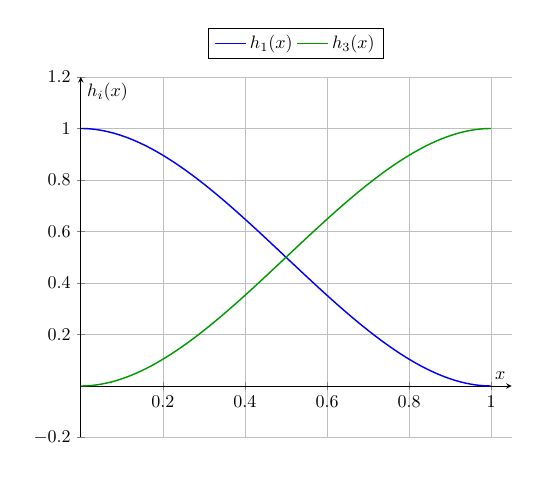
\begin{tikzpicture}[scale=0.65]
        \begin{axis}[
            axis lines=middle,
            xlabel={$x$},
            ylabel={$h_i(x)$},
            xmin=0, xmax=1.05,
            ymin=-0.2, ymax=1.2,
            grid=both,
            legend style={at={(0.5,1.05)}, anchor=south, legend columns=2},
            samples=200,
            domain=0:1
          ]
          % h1(x) = (2x^3 - 3x^2 + 1)
          \addplot[blue, thick] {2*x^3 - 3*x^2 + 1};
          \addlegendentry{$h_1(x)$}
          % h3(x) = (-2x^3 + 3x^2)
          \addplot[green!60!black, thick] {-2*x^3 + 3*x^2};
          \addlegendentry{$h_3(x)$}
        \end{axis}
      \end{tikzpicture}
      \textbf{Translational shape functions}

    \end{column}

    \begin{column}{0.45\textwidth}
      \centering
      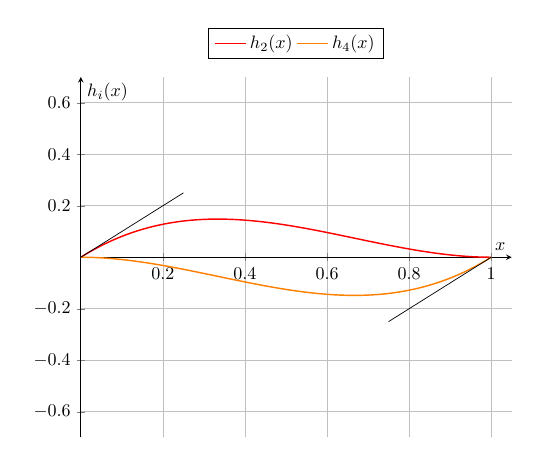
\begin{tikzpicture}[scale=0.65]
        \begin{axis}[
            axis lines=middle,
            xlabel={$x$},
            ylabel={$h_i(x)$},
            xmin=0, xmax=1.05,
            ymin=-0.7, ymax=0.7,
            grid=both,
            legend style={at={(0.5,1.05)}, anchor=south, legend columns=2},
            samples=200,
            domain=0:1
          ]
          % h2(x) = (x^3 - 2x^2 + x)
          \addplot[red, thick] {x^3 - 2*x^2 + x};
          \addlegendentry{$h_2(x)$}
          % h4(x) = (x^3 - x^2)
          \addplot[orange, thick] {x^3 - x^2};
          \addlegendentry{$h_4(x)$}
          % Tangent to h2 at x = 0: y = x, domain near 0
          \addplot[black, domain=0:0.25] {x};
          % Tangent to h4 at x = 1: y = x - 1, domain near 1
          \addplot[black, domain=0.75:1] {x - 1};
        \end{axis}
      \end{tikzpicture}
      \textbf{Rotational shape functions}
    \end{column}
  \end{columns}
\end{frame}


{\setbeamercolor{background canvas}{bg=darkred}
\setbeamercolor{block body}{bg=darkred,fg=white}
\setbeamercolor{itemize item}{fg=white}
\setbeamercolor{itemize/enumerate body}{fg=white}
\color{white}
\begin{frame}{Element stiffness matrix}
  \vspace{-0.5cm}

  \begin{align*}
    \mathbf{K} & =\int_0^{\ell}  EI\ \mathbf{B}^T\mathbf{B}\ dx                                                                                                                                                                                                                                                                \\
               & =\int_0^{\ell} EI \begin{bmatrix} (h_1^{\prime\prime})^2 & h_1^{\prime\prime} h_2^{\prime\prime} & h_1^{\prime\prime} h_3^{\prime\prime} & h_1^{\prime\prime} h_4^{\prime\prime} \\
                                       & (h_2^{\prime\prime})^2                & h_2^{\prime\prime} h_3^{\prime\prime} & h_2^{\prime\prime} h_4^{\prime\prime} \\ & & (h_3^{\prime\prime})^2                & h_3^{\prime\prime} h_4^{\prime\prime} \\ Symm. & & & (h_4^{\prime\prime})^2\end{bmatrix} \ dx \\[5pt]
               & =\frac{EI}{\ell^3} \begin{bmatrix} 12 & 6\ell & -12 & 6\ell \\  & 4\ell^2 & -6\ell & 2\ell^2\\ & &12 & -6\ell \\Symm. & & & 4\ell^2 \end{bmatrix}
  \end{align*}

  The deformation matrix is
  $$\mathbf B=\frac{d^2 \mathbf H}{dx^2}=\begin{bmatrix} h_1^{\prime\prime}(x) & h_2^{\prime\prime}(x) & h_3^{\prime\prime}(x) & h_4^{\prime\prime}(x) \end{bmatrix}$$
\end{frame}

\begin{frame}{Element consistent mass matrix}
  \vspace{-0.5cm}

  \begin{align*}
    \mathbf{M} & =\int_0^{\ell}  \rho A\ \mathbf{H}^T\mathbf{H}\ dx                                                                                           \\
               & =\int_0^{\ell} \rho A \begin{bmatrix} (h_1)^2 & h_1 h_2 & h_1 h_3 & h_1 h_4 \\
                        & (h_2)^2 & h_2 h_3 & h_2 h_4 \\ & & (h_3)^2                & h_3 h_4 \\ Symm. & & & (h_4)^2\end{bmatrix} \ dx \\[5pt]
               & =\frac{\rho A\ell }{420}\begin{bmatrix}
                                           156   & 22\ell  & 54     & -13\ell  \\
                                                 & 4\ell^2 & 13\ell & -3\ell^2 \\
                                                 &         & 156    & -22\ell  \\
                                           Symm. &         &        & 4\ell^2  \\
                                         \end{bmatrix}
  \end{align*}
\end{frame}

\begin{frame}{Element lumped mass matrix}
  \begin{itemize}
    \item Assumption that the mass of the structure is lumped at the nodal coordinates where translational displacements are defined.
    \item Inertial effect associated with any rotational degree of freedom is usually assumed to be zero.
    \item Recall that $\rho\, A$ is the mass per unit length along the beam, then the lumped mass matrix is defined as
          \vspace{0.3cm}
          $$\mathbf{M}=\frac{\rho A\ell}{2}\begin{bmatrix}
              1 & 0 & 0 & 0 \\
              0 & 0 & 0 & 0 \\
              0 & 0 & 1 & 0 \\
              0 & 0 & 0 & 0 \\
            \end{bmatrix}$$
  \end{itemize}
\end{frame}
}

\begin{frame}{Applied loads}
  \begin{itemize}
    \item \textbf{Uniformly distributed load:}
          \noindent
          \begin{columns}
            \begin{column}{0.55\textwidth}
              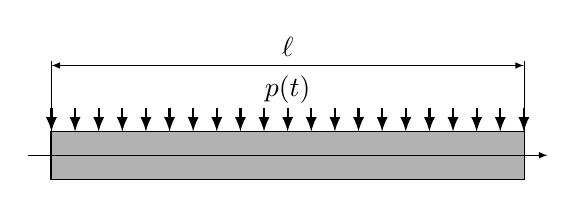
\begin{tikzpicture}[scale=0.6]
                \filldraw[fill=gray!60, draw=black,thick] (0,0) rectangle (10,1);
                % Draw the rectangle
                \fill[gray!60] (0,0) rectangle (10,1);
                % Add the p vector
                \foreach \i in {0,...,20}
                  {
                    \draw[-latex, thick]  (0.5*\i,1.5)--(0.5*\i,1);
                  }
                \node at (5,1.9) {\(p(t)\)};
                %axis
                \draw[-latex, ultra thin] (-0.5,0.5) -- (10.5,0.5);
                % length
                \draw[ultra thin] (10,0) -- (10, 2.5) ;
                \draw[ultra thin] (0,0) -- (0, 2.5) ;
                \draw[latex-latex, ultra thin]  (0,2.4)  to node[sloped,midway,above] {$\ell$}(10,2.4) ;
              \end{tikzpicture}
            \end{column}
            \begin{column}{0.45\textwidth}
              $$\mathbf r=\int_0^\ell p(t)\, \mathbf H^T\ dx=\dfrac{p(t)\ell}{2}\begin{bmatrix}
                  1      \\
                  \ell/6 \\
                  1      \\
                  -\ell/6
                \end{bmatrix}$$
            \end{column}
          \end{columns}
          \vspace{0.2cm}
          An uniform transverse load can be replaced by two equivalent transverse nodes loads of value $(p\ell)/2$ and by two equivalent nodal moments of values $\pm p\ell^2/12$.
          \vspace{0.2cm}

    \item \textbf{Concentrated loads:}
          \noindent
          \begin{columns}
            \begin{column}{0.48\textwidth}
              \centering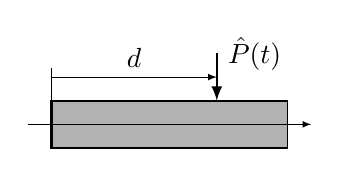
\begin{tikzpicture}[scale=0.6]
                \draw[fill=gray!60] (0,0) rectangle (5,1);
                % Draw the rectangle
                \draw[thick] (5,1) -- (0,1) -- (0,0) -- (5,0);
                % Add the p vector
                \draw[-latex, thick]  (3.5,2)--(3.5,1);
                \node at (4.3,2) {\(\hat P(t)\)};
                %axis
                \draw[-latex, ultra thin] (-0.5,0.5) -- (5.5,0.5);
                % x
                \draw[, ultra thin] (0,0) -- (0,1.7);
                \draw[-latex,ultra thin] (0,1.5) to node[midway,above] {$d$} (3.5,1.5);
              \end{tikzpicture}
              $$\mathbf r(t)=\hat P(t)\, \mathbf H^T(d)$$
            \end{column}
            \begin{column}{0.48\textwidth}
              \centering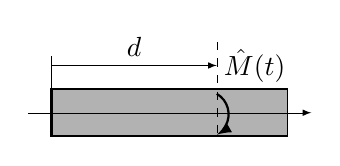
\begin{tikzpicture}[scale=0.6]
                \draw[fill=gray!60] (0,0) rectangle (5,1);
                % Draw the rectangle
                \draw[thick] (5,1) -- (0,1) -- (0,0) -- (5,0);
                % Add the p vector
                \draw[-latex, thick] (3.5,0.9) arc (60:-60:0.5);
                \draw[ultra thin, dashed]  (3.5,2)--(3.5,-0);
                \node at (4.3,1.5) {\(\hat M(t)\)};
                %axis
                \draw[-latex, ultra thin] (-0.5,0.5) -- (5.5,0.5);
                % x
                \draw[, ultra thin] (0,0) -- (0,1.7);
                \draw[-latex,ultra thin] (0,1.5) to node[midway,above] {$d$} (3.5,1.5);
              \end{tikzpicture}
              $$\mathbf r(t)=\hat M(t)\, \frac{d\mathbf H}{dx}^T(d)$$
            \end{column}
          \end{columns}
  \end{itemize}
\end{frame}

\begin{frame}{Post-processing: approximation of bending moment and shear force}
  \begin{itemize}
    \item The approximated bending moment along the beam element is
          \vspace{0.2cm}
          $$M^h(x,t)=EI\partial_{xx}^2u_{2}^h(x,t)=EI\, \mathbf B(x)\mathbf q(t).$$
          \vspace{-0.3cm}
    \item The approximated shear force along the beam element is
          \vspace{0.2cm}
          $$V^h(x,t)=-\partial_xM^h(x,t)=-EI\, \frac{d\mathbf B}{dx}(x)\mathbf q(t).$$
  \end{itemize}
\end{frame}

\begin{frame}{MATLAB examples}
  \begin{itemize}
    \item A Cantilever beam subjected to a downward force
    \item A clamped-clamped beam in free vibration.
  \end{itemize}

  \begin{center}
    \href{https://drive.mathworks.com/sharing/6a9792ef-d0a7-4aca-a1d0-8b1862b0ac3b}{\beamergotobutton{Go to Matlab Drive}}
  \end{center}
\end{frame}

\section{Geometric stiffness}

\begin{frame}{Beam subjected to axial loads}
  \begin{itemize}
    \item Consider a beam subjected to axial forces $N$ applied at both ends.
  \end{itemize}
  \begin{center}
    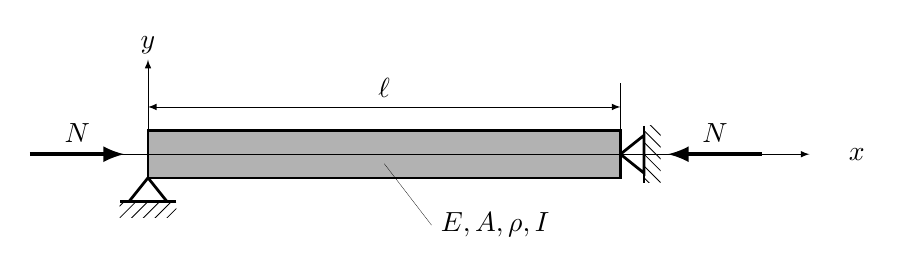
\begin{tikzpicture}[scale=0.6]
      \point{a}{0}{0};
      \point{b}{6}{0.5*0.6};
      \support {1}{a}[0];
      \support {1}{b}[90];
      % Draw the rectangle
      \filldraw[fill=gray!60, draw=black,thick] (0,0) rectangle (10,1);
      %axis
      \draw[-latex, ultra thin] (-1,0.5) -- (14,0.5);
      \draw[-latex, ultra thin] (0,0) -- (0,2.5);
      \node at (15,0.5) {\(x\)};
      \node at (0,2.8) {\(y\)};
      % length
      \draw[ultra thin] (10,0) -- (10, 2) ;
      \draw[latex-latex, ultra thin]  (0,1.5)  to node[sloped,midway,above] {$\ell$}(10,1.5) ;
      % N
      \draw[latex-, ultra thick] (11,0.5) -- (13,0.5) node[midway, above]{$N$};
      \draw[-latex, ultra thick] (-2.5,0.5) -- (-0.5,0.5) node[midway, above]{$N$};
      \draw[ultra thin]  (5,0.3) -- (6,-1) node[right]{$E,A,\rho,I$};
    \end{tikzpicture}
  \end{center}
  \begin{itemize}
    \item Beam carrying large axial loads or undergoing large displacements have nonlinear behavior arising from the internal moments that are the product of the axial loads and the displacements transverse to the loads.
    \item The stiffness coefficients $k_{ij}$ must be modified by the presence of the axial force to the corresponding \textbf{geometric stiffness coefficients} $k^g_{ij}$.
  \end{itemize}
\end{frame}

\begin{comment}
\begin{frame}{Geometric stiffness matrix}
  \begin{block}{}
    For frame elements with transverse rotation $\theta_3(x,t)$, but without displacements along the axial coordinate $x$ the frame element undergoes axial deformation $u_1(x,t)$.
  \end{block}
  \vspace{0.3cm}
  \begin{columns}
    \begin{column}{.45\textwidth}
      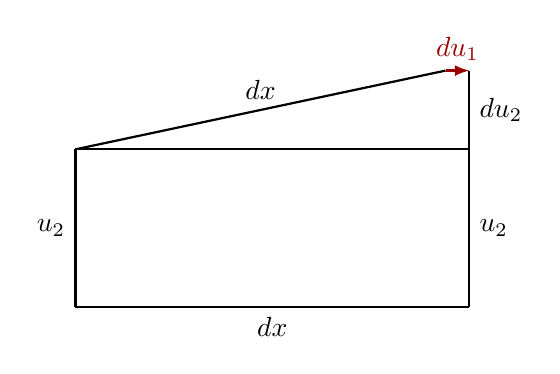
\begin{tikzpicture}
        \draw[thick] (0,0) -- (5,0) node[midway, below]{$dx$};
        \draw[thick] (5,0) -- (5,2) node[midway, right]{$u_2$};
        \draw[thick] (5,2) -- (5,3) node[midway, right]{$du_2$};
        \draw[thick] (0,0) -- (0,2) node[midway, left]{$u_2$};
        \draw[thick] (0,2) -- (5,2);
        \draw[thick] (0,2) -- (4.7,3) node[midway, above]{$dx$};
        \draw[thick,-latex,darkred] (4.7,3) -- (5,3) node[midway, above]{$du_1$};
      \end{tikzpicture}    \end{column}
    \begin{column}{.45\textwidth}
      Using the Pythagorean theorem:
      $$dx^2=(dx-du_1)^2+du_2^2$$
      $$\frac{du_1}{dx}=\frac{1}{2}\left(\frac{du_1}{dx}\right)^2+\frac{1}{2}\left(\frac{du_2}{dx}\right)^2$$
      Axial strain is less than transverse rotations:
      $$\frac{du_1}{dx}\approx \frac{1}{2}\left(\frac{du_2}{dx}\right)^2$$
    \end{column}
  \end{columns}
\end{frame}


\begin{frame}{Geometric stiffness matrix}
  \begin{itemize}
    \item Strain energy associated with axial forces $N(x)$ and axial geometric deformation
          \[
            U_G = \int_0^\ell N(x) \frac{du_1(x)}{dx} \, dx = \frac{1}{2} \int_0^L N(x) \left( \frac{du_2(x)}{dx} \right)^2 dx.
          \]
    \item Employing the approximation $u_2^h(x,t)=\mathbf H(x)\mathbf q(t)$ yield to
          \[
            U_G = \frac{1}{2} \mathbf q^T\int_0^L N(x) \frac{d\mathbf H}{dx}^T\frac{d\mathbf H}{dx}\,  dx \ \mathbf q.
          \]
    \item The geometric stiffness matrix is defined as
          $$\mathbf K^g=\int_0^\ell N(x)\, \frac{d\mathbf H}{dx}^T\frac{d\mathbf H}{dx}\ dx$$
  \end{itemize}
\end{frame}
\end{comment}

\begin{frame}{Geometric stiffness matrix}
  \begin{block}{}
    $k^g_{ij}$ is defined as the force corresponding to the nodal coordinate $i$ due to a unit displacement at coordinate $j$ and resulting for the axial force $N$.
  \end{block}
  \textbf{Calculation of $k^g_{12}$}: vertical force at node 1 due to a unit rotation $\theta_2=1$ caused by the axial force $N$. May be evaluated by the principle of virtual work:
  \vspace{0.3cm}
  \begin{columns}
    \begin{column}{.45\textwidth}
      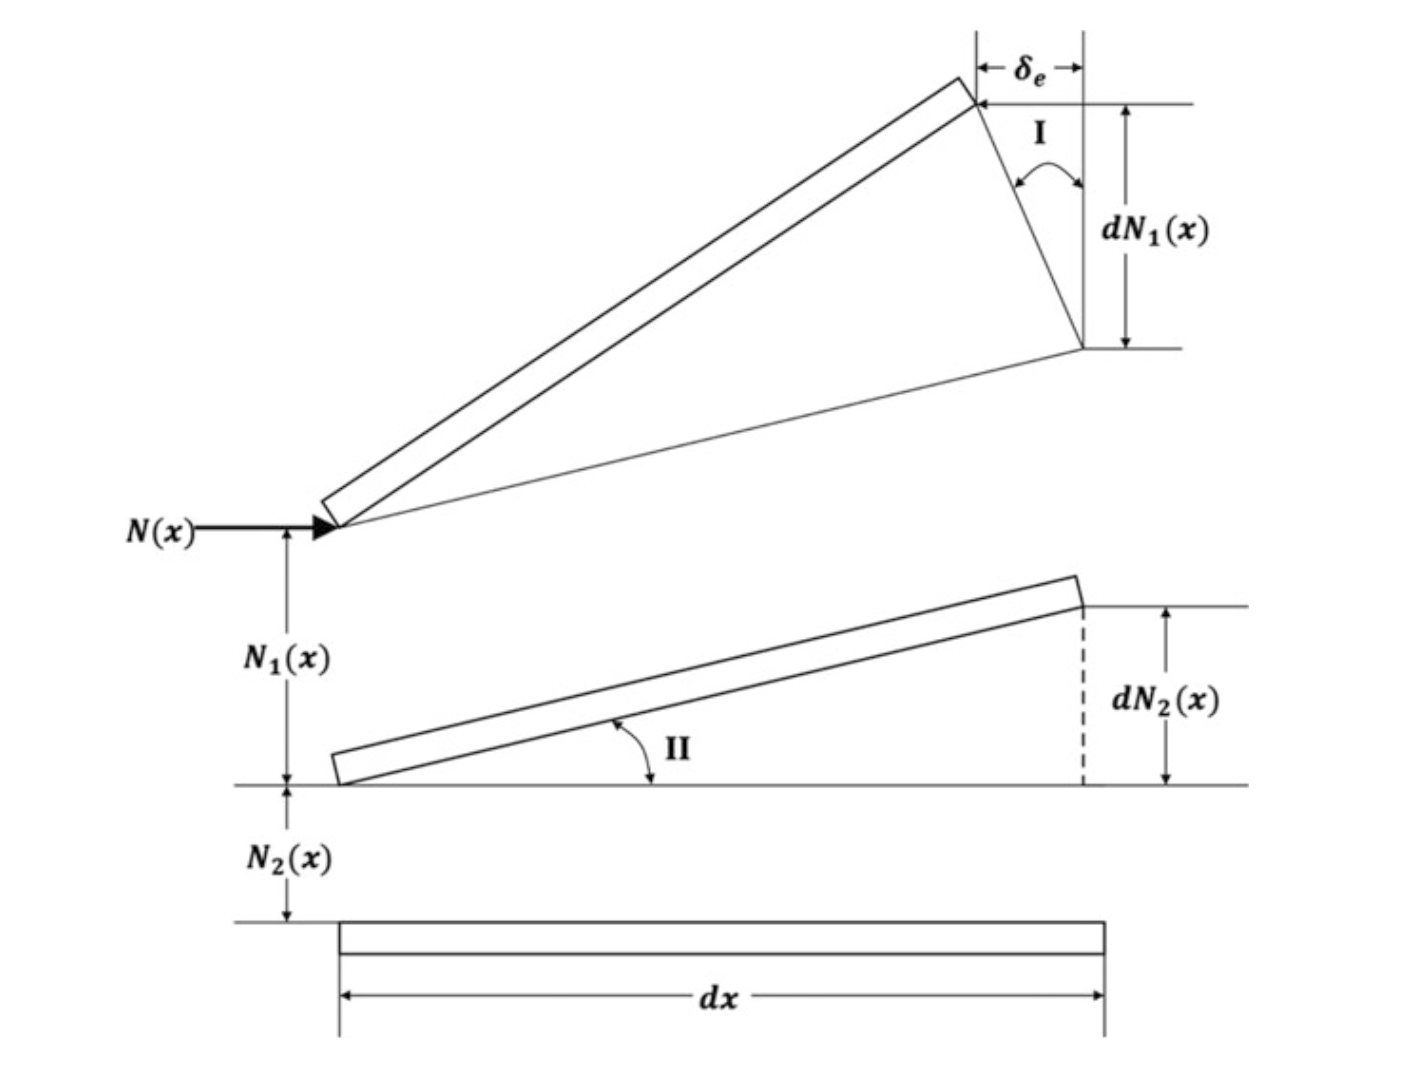
\includegraphics[width=4.5cm]{../images/geometricStiffness.png}
    \end{column}
    \begin{column}{.45\textwidth}
      $$dW=N\delta_e$$
      By similar triangles we have
      \begin{align*}
        \frac{\delta_e}{dh_1(x)} & =\frac{dh_2(x)}{dx}                         \\
        \delta_e                 & = \frac{dh_1}{dx}(x)\frac{dh_2}{dx}(x)\, dx
      \end{align*}
    \end{column}
  \end{columns}
  $$k^g_{12}=N\int_0^\ell h_1^\prime(x)h_2^\prime(x)\, dx$$
\end{frame}

\begin{frame}{Geometric stiffness matrix}
  \begin{itemize}
    \item In general, any geometric stiffness coefficient may be expressed as
          $$k^g_{ij}=N \int_0^\ell h_i^\prime(x)h_i^\prime(x)\, dx$$
    \item We define the \textbf{geometric stiffness matrix} as:
          $$\mathbf K^g=N\int_0^\ell \, \frac{d\mathbf H}{dx}^T\frac{d\mathbf H}{dx}\ dx$$
    \item When $N$ is constant along the beam length we obtain
          $$\mathbf K^g=\frac{N}{30\ell}\begin{bmatrix}
              36    & 3\ell   & -36    & 3\ell   \\
              3\ell & 4\ell^2 & -3\ell & -\ell^2 \\
              -36   & -3\ell  & 36     & -3\ell  \\
              3\ell & -\ell^2 & -3\ell & 4\ell^2 \\
            \end{bmatrix}
          $$
  \end{itemize}
\end{frame}

\begin{frame}{Example: stability of Bernoulli beam}
  \begin{center}
    \href{https://drive.mathworks.com/sharing/6a9792ef-d0a7-4aca-a1d0-8b1862b0ac3b}{\beamergotobutton{Go to Matlab Drive}}
  \end{center}
\end{frame}

\section{Timoshenko planar beam}

\begin{frame}{Higher-order deformation theories for beams}
  \begin{columns}
    \begin{column}{0.3\textwidth}
      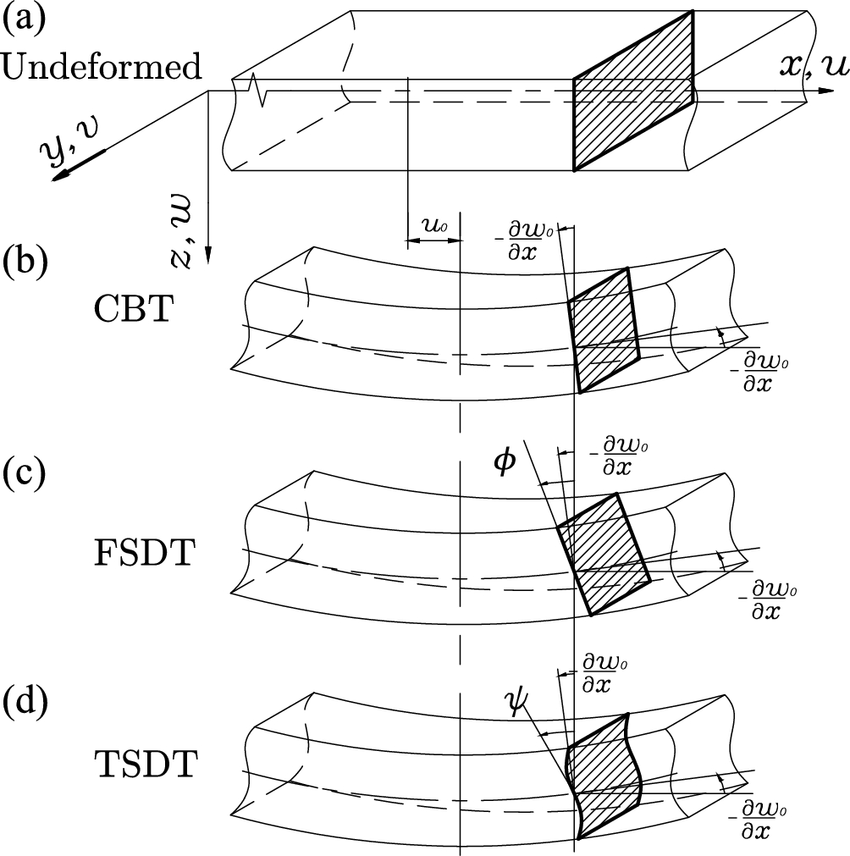
\includegraphics[width=4.5cm]{../images/higherDefTheories.png}
    \end{column}
    \small
    \begin{column}{0.7\textwidth}
      \begin{itemize}
        \item \textbf{Classical beam theory} (Euler-Bernoulli) is a zero-order shear deformation theory.
        \item \textbf{Timoshenko theory} is a first-order shear deformation theory. Cross-sectional planes remain straight but not necessarily perpendicular to the mid-surface.
              \begin{itemize}
                \item Displacements are linear functions through thickness.
                \item In-plane strains are linear in $z$.
                \item Shear strains are constant in $z$.
              \end{itemize}
        \item  \textbf{Third-order shear deformation theory}: normal cross-sectional planes to the mid-surface can rotate and deform.
              \begin{itemize}
                \item Displacements are cubic functions through thickness.
                \item In-plane strains are cubic in $z$.
                \item Shear strains are quadratic in $z$.
              \end{itemize}
      \end{itemize}
    \end{column}
  \end{columns}
\end{frame}

\begin{frame}
  \frametitle{Kinematic assumptions for planar Timoshenko beam}
  \begin{enumerate}
    \item The beam dynamics will be restricted to the $O(x,y)$ plane.
    \item The beam cross-section remains planar after deformation.
    \item Lines that are straight and perpendicular to the geometrical beam axis remain straight but \textbf{not necessarily perpendicular} during deformation.
  \end{enumerate}

  \begin{columns}
    \column{0.6\textwidth}
    \begin{center}
      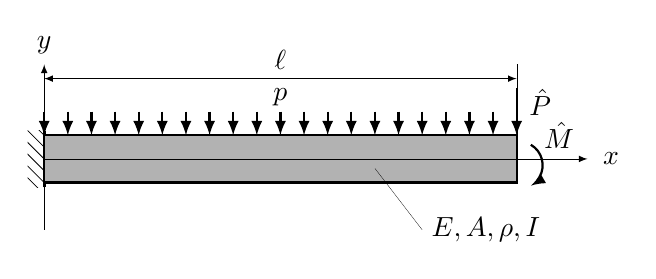
\begin{tikzpicture}[scale=0.6]
        \point{a}{0}{0.3};
        \support {3}{a}[270];
        % Draw the rectangle
        \filldraw[fill=gray!60, draw=black,thick] (0,0) rectangle (10,1);
        % Add the p vector
        \foreach \i in {0,...,19}
          {
            \draw[-latex, thick]  (0.5*\i,1.5)--(0.5*\i,1);
          }
        \node at (5,1.8) {\(p\)};
        %axis
        \draw[-latex, ultra thin] (0,0.5) -- (11.5,0.5);
        \draw[-latex, ultra thin] (0,-1) -- (0,2.5);
        \node at (12,0.5) {\(x\)};
        \node at (0,2.9) {\(y\)};
        % length
        \draw[ultra thin] (10,0) -- (10, 2.5) ;
        \draw[latex-latex, ultra thin]  (0,2.2)  to node[sloped,midway,above] {$\ell$}(10,2.2) ;
        % M and V 
        \draw[-latex, thick] (10.3,0.8) arc (60:-60:0.5);
        \node at (10.5,1.7) {\(\hat P\)};
        \draw[-latex, thick] (10,2) -- (10,1);
        \node at (10.9,1) {\(\hat M\)};
        \draw[ultra thin]  (7,0.3) -- (8,-1) node[right]{$E,A,\rho,I$};
      \end{tikzpicture}
    \end{center}
    \column{.25\textwidth}
    {\tiny Model parameters:
      \begin{itemize}\setlength\itemsep{0.05em}
        \item $A$ cross-sectional area
        \item $E$ Young's modulus
        \item $\rho$ material density
        \item $I$ moment of inertia
        \item $\ell$ length
      \end{itemize}}
    \column{.25\textwidth}
    {\tiny Loads:
      \begin{itemize}\setlength\itemsep{0.05em}
        \item  $\hat M$  bending moment \\ at free end
        \item  $\hat P$ load at \\ free end
        \item $p$ distributed transversal load
      \end{itemize}
    }
  \end{columns}
  \begin{block}{Variables:}
    \begin{multicols}{2}
      \begin{itemize}\setlength\itemsep{0.05em}
        \item $u_{1}(x,t)$ axial displacement
        \item $u_{2}(x,t)$ transversal displacement\vspace{.1cm}
      \end{itemize}
    \end{multicols}
  \end{block}
\end{frame}


\begin{frame}
  \frametitle{Displacements field}
  Introduce an auxiliary variable $\theta_{3}(x,t)$ representing the total rotation of the section around the $Oz$ axis. Rotations are positive in clockwise direction.
  \begin{columns}
    \column{0.35\textwidth}
    \begin{center}
      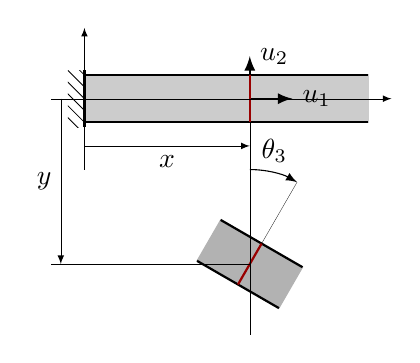
\begin{tikzpicture}[scale=0.6]
        \point{a}{0}{0.3};
        \support {3}{a}[270];
        % Draw the rectangle
        \filldraw[fill=gray!40, draw=gray!40,thick] (0,0) rectangle (6,1);
        \draw[thick](6,1)-- (0,1) -- (0,0)--(6,0);
        \draw[-latex,thick] (3.5,0.5) -- (4.4,.5) node[right]{$u_{1}$};
        \draw[-latex,thick] (3.5,0.5) -- (3.5,1.4) node[right]{$u_{2}$};
        \draw[darkred,thick] (3.5,0) -- (3.5,1);
        %deformed 
        \filldraw[fill=gray!60,draw=gray!60, rotate around={-30:(3.5,-3)}] (2.5,-2.5) rectangle (4.5,-3.5);
        \draw[thick,rotate around={-30:(3.5,-3)},shift={(0,-0.5)}](2.5,-3)-- (4.5,-3);
        \draw[thick,rotate around={-30:(3.5,-3)},shift={(0,0.5)}](2.5,-3)-- (4.5,-3);
        \draw[ultra thin,rotate around={-30:(3.5,-3)}](3.5,-3)-- (3.5,-1);
        \draw[darkred,thick,rotate around={-30:(3.5,-3)}](3.5,-2.5)-- (3.5,-3.5);
        \draw[-latex] (3.5,-1) arc (90:60:2) node[midway,above] {$\theta_{3}$};
        %x1 and x2
        \draw[ultra thin] (3.5,-0.7) -- (3.5,0);
        \draw[-latex,ultra thin] (0,-0.5) to node[midway,below] {$x$} (3.5,-.5);
        \draw[ultra thin]  (-.7,-3)-- (3.5,-3);
        \draw[ultra thin] (3.5,-4.5) -- (3.5,-0.5);
        \draw[ultra thin] (-.7,0.5) -- (0,0.5);
        \draw[-latex,ultra thin] (-.5,.5) to node[midway,left] {$y$} (-.5,-3);
        %axis
        \draw[ultra thin,-latex] (0,0.5) -- (6.5,0.5);
        \draw[ultra thin,-latex] (0,-1) -- (0,2);
      \end{tikzpicture}
    \end{center}
    \column{0.7\textwidth}

    \begin{itemize}
      \item The first Timoshenko assumption implies
            $$u_3=0.$$
      \item The second Timoshenko assumption implies
            $$u_{1}=-y\theta_{3}\qquad\qquad\text{\emph{(rotation-axial displ.)}}$$
            %Notice, that because the convention of positive rotations in the counterclockwise directions, the term has a negative sign. In this way, is assured that a positive value of rotation will create a negative axial displacement for a positive $y$.
    \end{itemize}
  \end{columns}
  \begin{block}{}
    \textbf{Two unknowns:} $u_{2}(x,t)$ transversal displacement and $\theta_{3}(x,t)$ rotation of the section around the $Oz$ axis.
  \end{block}
\end{frame}

\begin{frame}
  \frametitle{Stress, strain and displacement fields}
  \begin{block}{Strain-displacement relationships}
    Substituting the displacement field $\mathbf u$ into $\boldsymbol{\varepsilon}=\nabla\mathbf u$ yield to :
    \vspace{-0.6cm}

    \begin{align*}
      \varepsilon_{11}                      & =\partial_{x}u_{1}=-y\partial_{xx}^2u_{2}                                                & \textcolor{darkred}{\varepsilon_{22}} & \textcolor{darkred}{\ =\partial_{y}u_{2}} \\
      \textcolor{darkred}{\varepsilon_{12}} & \textcolor{darkred}{\ =\partial_{x}u_{2}+\partial_{y}u_{1}=\partial_{x}u_{2}-\theta_{3}} & \quad \varepsilon_{33}                & = \varepsilon_{23} = \varepsilon_{13} = 0
    \end{align*}
  \end{block}
  \begin{block}{Generalized Hooke's law}
    Using the linear relationship for homogeneous and isotropic material,
    $\boldsymbol\sigma=\mathbf C\boldsymbol\varepsilon$, is possible to write the stress field in term of the strain field as :
    \vspace{-0.6cm}

    \begin{align*}
      \sigma_{11}                      & =(\lambda + 2G)\varepsilon_{11}            &
      \textcolor{darkred}{\sigma_{12}} & \textcolor{darkred}{\ =2G\varepsilon_{12}}   \\
      \sigma_{22}                      & =\sigma_{33}=\lambda \varepsilon_{11}      &
      \sigma_{13}                      & = \sigma_{23} = 0
    \end{align*}

    where $\lambda=\frac{E}{(1+\nu)(1-2\nu)}$ and the shear modulus $G=\frac{E}{2(1+\nu)}$ are Lamé constants.
  \end{block}
\end{frame}

\begin{frame}{Dynamic equilibrium equations}
  \begin{block}{Additional assumptions regarding the stress field}
    $$\sigma_{11}  = E\varepsilon_{11},\quad \sigma_{12} =2G\varepsilon_{12} \qquad\text{and}\qquad
      \sigma_{22}  =  \sigma_{33}  = \sigma_{13} = \sigma_{23} = 0.
    $$
    % since the dimension of the cross-section of the beam is much smaller that the length of the beam
  \end{block}

  \begin{columns}
    \column{0.5\textwidth}
    \begin{center}
      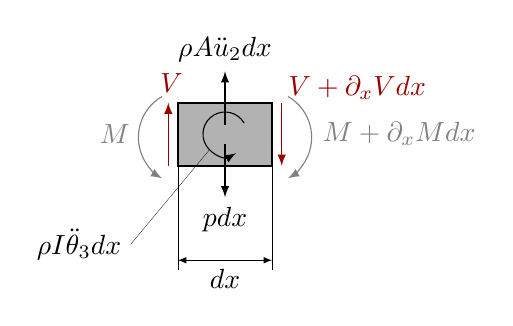
\begin{tikzpicture}[scale=0.4]
        % Draw the rectangle
        \filldraw[fill=gray!60, draw=black,thick] (0,0) rectangle (3,2);
        %axis
        \draw[ultra thin] (0,0) -- (0,-3.3);
        \draw[ultra thin] (3,0) -- (3,-3.3);
        \draw[latex-latex,ultra thin] (0,-3) to node[midway,below] {$dx$} (3,-3);
        \draw[-latex]  (1.5,1.3)  -- (1.5,3) node[above] {$\rho A\ddot u_{2}dx$};
        \draw[-latex]  (1.5,.7)  -- (1.5,-1) node[below] {$pdx$};
        \draw[gray,-latex] (-0.5,2.2) arc (120:240:1.5);
        %M vactors 
        \node[gray] at (-2,1) {\(M\)};
        \draw[gray,-latex] (3.5,2.2) arc (60:-60:1.5);
        \draw (4.3,1) node[gray,right] {$M+\partial_{x}Mdx$};
        % Add the V vectors
        \draw[darkred,-latex] (-0.3,0) -- (-0.3,2);
        \node[darkred,above] at (-0.2,2) {\(V\)};
        \draw[darkred,latex-] (3.3,0) -- (3.3,2);
        \node[darkred,above] at (5.7,1.8) {\(V+\partial_{x}Vdx\)};
        % Rotatory inertia
        \draw[ultra thin] (1,0.5) -- (-1.5,-2.5) node[left]{$\rho I\ddot \theta_{3}dx$};
        \draw[latex-] (1.85,.4) arc (300:30:0.7);
      \end{tikzpicture}
    \end{center}
    \column{0.6\textwidth}
    \vspace{-0.2cm}
    \begin{itemize}
      \item Equilibrium of transverse forces:
            $$ \partial_{x}{\color{darkred}V}+p =\rho A\ddot u_{2}  $$
      \item Equilibrium of moments:
            $$ \partial_{x}{\color{gray}M}+{\color{darkred}V}=\rho I\ddot \theta_{3}$$
    \end{itemize}

  \end{columns}\vspace{-0.3cm}
  \begin{align*}
    {\color{darkred}V} & =\int_{A}\sigma_{12}\, dA=kGA\varepsilon_{12}={\color{darkred} kGA(\partial_{x}u_{2}-\theta_{3})}    \\
    {\color{gray}M}    & =-\int_{A} y\sigma_{11}\, dA=-\int_{A}yE\varepsilon_{11}\, dA={\color{gray}EI\partial_{x}\theta_{3}} \\
  \end{align*}
\end{frame}


\begin{frame}
  \frametitle{Strong form for transversal vibrations for Timoshenko beam}
  \vspace{-0.5cm}
  The weak formulation of the problem consists of finding the transversal displacement $u_{2}\in C^2([0,\ell]\times[0,T])$ and the rotation $\theta_{3}\in C^2([0,\ell]\times[0,T])$ such that the following equilibrium equations, boundary and initial conditions are satisfied.
  \begin{block}{}
    \vspace{-.5cm}
    \begin{align*}
      \partial_{x}\big({\color{darkred}kGA(\partial_{x}u_{2}-\theta_{3})}\big)+p                                      & =\rho A\ddot u_{2}      \\
      \partial_{x}\big({\color{gray}EI\partial_{x}\theta_{3}}\big)+{\color{darkred}kGA(\partial_{x}u_{2}-\theta_{3})} & =\rho I\ddot \theta_{3} \\
    \end{align*}
    \vspace{-1cm}\newline\small In matrix form: $\nabla_{\sigma}^{T}\mathbf C\nabla_{u}\mathbf u+\mathbf f=\mathbf {M \ddot u}$, where
    $$\underbrace{\begin{bmatrix}
          \partial_{x} & 0            \\
          1            & \partial_{x}
        \end{bmatrix}}_\text{$\nabla_{\sigma}^{T}$}
      \underbrace{\begin{bmatrix}
          kGA & 0  \\
          0   & EI
        \end{bmatrix}}_\text{$\mathbf C$}
      \underbrace{\begin{bmatrix}
          \partial_{x} & -1           \\
          0            & \partial_{x}
        \end{bmatrix}}_\text{$\nabla_{u}$}
      \underbrace{\begin{bmatrix}
          u_{2} \\
          \theta_{3}
        \end{bmatrix}}_\text{$\mathbf u$}
      +
      \underbrace{\begin{bmatrix}
          p \\
          0
        \end{bmatrix}}_\text{$\mathbf f$}
      =
      \underbrace{\begin{bmatrix}
          \rho A & 0      \\
          0      & \rho I
        \end{bmatrix}}_\text{$\mathbf M$}
      \underbrace{\begin{bmatrix}
          \ddot u_{2} \\
          \ddot \theta_{3}
        \end{bmatrix}}_\text{$\mathbf{\ddot u}$}
    $$
  \end{block}
\end{frame}

\begin{frame}
  \begin{block}{Boundary conditions}
    \begin{columns}
      \column{0.4\textwidth}
      \[
        \begin{aligned}
           & u_2(0, t) = 0 \quad        &  & \\
           & \theta_{3}(0, t) = 0 \quad &  & \\
        \end{aligned}
      \]
      \column{0.6\textwidth}
      \[
        \begin{aligned}
           & kGA \big(\partial_{x}u_{2}(\ell, t)-\theta_{3}(\ell, t) \big)= \hat P &  & \\
           & EI \partial_{x}\theta_{3}(\ell, t)=\hat M                             &  & \\
        \end{aligned}
      \]
    \end{columns}
    \vspace{.2cm}\small In matrix form: let $\hat{\mathbf{f}}=[\hat P,\, \hat M]^T$ then
    $$\begin{aligned}
        \mathbf u(0,t)                        & =\mathbf 0       \\
        \mathbf C\nabla_{u} \mathbf u(\ell,t) & =\mathbf{\hat f} \\
      \end{aligned}$$
  \end{block}

  \begin{block}{Initial conditions}
    \begin{columns}
      \column{0.5\textwidth}
      \[
        \begin{aligned}
           & u_2(x, 0) = u_{0}(x) \quad             &  & \\
           & \theta_{3}(x, 0) = \theta_{0}(x) \quad &  & \\
        \end{aligned}
      \]
      \column{0.5\textwidth}
      \[
        \begin{aligned}
           & \dot u_2(x, 0) = v_{0}(x) \quad           &  & \\
           & \dot \theta_{3}(x, 0) = \phi_{0}(x) \quad &  & \\
        \end{aligned}
      \]
    \end{columns}
    \vspace{.2cm}\small In matrix form:  $\mathbf{u_{0}}=[u_0,\, \theta_0]^T$ and $\mathbf{v_{0}}=[v_0,\, \phi_0]^T$ then
    $$\begin{aligned}
        \mathbf u(x,0)       & =\mathbf{u_{0}} \\
        \mathbf{\dot u}(x,0) & =\mathbf{v_{0}}
      \end{aligned}$$
  \end{block}
\end{frame}

\begin{frame}
  \frametitle{Weak form for transversal vibrations for Timoshenko beam}
  The weak formulation of the problem consists in finding the unknown function $\mathbf{u} \in \mathcal U$ which satisfies the equation $\forall \boldsymbol\delta \mathbf{u} \in \mathcal{V}$:
  $$
    \begin{aligned}
       & \int_0^{\ell}\left(\nabla_u \boldsymbol\delta \mathbf{u}\right)^{\mathrm{T}} \mathbf{C}\left(\nabla_u \mathbf{u}\right) \mathrm{d} x+\int_0^{\ell} \boldsymbol\delta \mathbf{u}^{\mathrm{T}} \mathbf{M} \ddot{\mathbf{u}}\, d x =\int_0^{\ell} \boldsymbol\delta \mathbf{u}^{\mathrm{T}} \mathbf{f} d x+\boldsymbol\delta \mathbf{u}^{\mathrm{T}}(\ell)\mathbf{\hat f}.
    \end{aligned}
  $$
  The function spaces $\mathcal U$ and $\mathcal V$ are defined as follows
  $$
    \begin{aligned}
       & \mathcal U=\left\{\mathbf{u}=\left\{u_2, \theta_3\right\}^{\mathrm{T}} \mid u_2(\cdot,t) \in H^1(] 0, \ell[) ; \theta_3(\cdot,t) \in H^1(] 0, \ell[) ; u_2(0, t)=\theta_3(0, t)=0\right\},                                     \\
       & \mathcal V=\left\{\boldsymbol\delta \mathbf{u}=\left\{\delta u_2, \delta \theta_3\right\}^{\mathrm{T}} \mid \delta u_2 \in H^1(] 0, \ell[) ; \delta \theta_3 \in H^1(] 0, \ell[) ; \delta u_2(0)=\delta \theta_3(0)=0\right\}.
    \end{aligned}
  $$
\end{frame}

{\setbeamercolor{background canvas}{bg=darkred}
\setbeamercolor{block body}{bg=darkred,fg=white}
\setbeamercolor{itemize item}{fg=white}
\setbeamercolor{itemize/enumerate body}{fg=white}
\color{white}
\begin{frame}{Displacement approximation}
  \small
  \begin{itemize}
    \item We approximate the generalized displacement using the ansatz:
          \[            \mathbf u^{h}(\mathbf x,t) = \mathbf H(\mathbf x)\mathbf q(t)    \qquad \text{and} \qquad
            \delta\mathbf u^{h}(\mathbf x)  =\mathbf H(\mathbf x)\delta\mathbf q
          \]
    \item \textbf{Cubic shape functions} are used to approximate the transversal displacement and \textbf{linear shape functions} for the rotation field:
          $$
            \mathbf H=\left[
              \begin{array}{cccc}
                h^c_1 & h^c_2 & h^c_3 & h^c_4 \\[0.5em]
                0     & h^l_1 & 0     & h^l_2 \\
              \end{array} \right]
          $$
          \vspace{-0.1cm}
          \begin{align*}
            h^c_1(x) & =2(x/\ell)^3-3(x/\ell)^2+1 & h^c_3(x) & =3(x/\ell)^2-2(x/\ell)^3 \\
            h^c_2(x) & =x(1-x/\ell)^2             & h^c_4(x) & =x(x/\ell)(x/\ell-1)     \\
            h^l_1(x) & = 1-x/\ell                 & h^l_2(x) & = x/\ell
          \end{align*}
    \item $\mathbf q(t)$ is a vector of (\emph{unknown}) nodal displacements and  $\bolddelta \mathbf q$ is a vector of constants:
          $$\mathbf q(t)=\left[
              \begin{array}{cccc}
                q_{1y}(t) & \phi_{1z}(t) & q_{2y}(t) & \phi_{2z}(t)
              \end{array} \right]^T\qquad \text{and}\qquad\bolddelta\mathbf q=\left[\begin{array}{cccc}
                \delta q_{1y} & \delta \phi_{1z} & \delta q_{2y} & \delta \phi_{2z}
              \end{array}\right]^T$$
  \end{itemize}
\end{frame}

\begin{frame}{Deformation, stiffness, mass matrices and loads vector}
  \begin{itemize}
    \item $\mathbf B=\nabla_u\mathbf H$ is the deformation matrix:
          \begin{align*}
            \mathbf B
            =\left[
              \begin{array}{cccc}
                \partial_x{h_1^c} & \partial_x{h_2^c}-h_1^l & \partial_x{h_3^c} & \partial_x{h_4^c}-h_2^l \\
                0                 & \partial_x{h_1^l}       & 0                 & \partial_x{h_2^l}
              \end{array}\right]
          \end{align*}
    \item The stiffness $\mathbf K$ and mass $\mathbf{Ma}$ matrices and load vector $\mathbf r$ are defined as
          \begin{align*}
            \mathbf K    & =\int_0^\ell \mathbf B^T\mathbf C\mathbf B \, dx,                                   \\
            \mathbf{Ma}  & =\int_0^\ell \mathbf H^T\mathbf M\mathbf H \, dx,                                   \\
            \mathbf r(t) & = \int_{0}^{\ell} \mathbf H^{T}\mathbf f\, dx + \mathbf H^{T}(\ell)\mathbf{\hat f}.
          \end{align*}
    \item The semi-discrete equations of motion are given by
          $$\mathbf{Ma}\,\ddot{\mathbf q}(t)+\mathbf K\mathbf q(t)=\mathbf r(t).$$
  \end{itemize}
\end{frame}
}

\begin{frame}{MATLAB example - modal analysis of a Timoshenko beam}
  \begin{center}
    \href{https://drive.mathworks.com/sharing/6a9792ef-d0a7-4aca-a1d0-8b1862b0ac3b}{\beamergotobutton{Go to Matlab Drive}}
  \end{center}
\end{frame}
\end{document}